\documentclass{article}

\usepackage{neurips_2024}
\usepackage[utf8]{inputenc}
\usepackage[T1]{fontenc}
\usepackage{hyperref}
\usepackage{url}
\usepackage{booktabs}
\usepackage{amsfonts}
\usepackage{amsmath}
\usepackage{amssymb}
\usepackage{graphicx}
\usepackage{subcaption}
\usepackage{xcolor}
\usepackage{microtype}
\usepackage{cite}

\newcommand{\method}{TinySSL}

\title{\textbf{\method}: Distilling Foundation Model Features\\for Resource-Efficient Vision}

\author{
  Emran Abdu\\
  \texttt{jakeniel98@gmail.com}\\
  \href{https://x.com/Emran_py}{X: @Emran\_py} \quad
  \href{https://github.com/Emran-goat}{GitHub: Emran-goat} \quad
  \href{https://www.linkedin.com/in/emran-abdu-833981315/}{LinkedIn}
}

\begin{document}

\maketitle

\begin{abstract}
Vision foundation models like DINOv2 produce powerful representations, but training them costs millions of dollars in GPU compute. We introduce \method, a 2.8M-parameter framework that distills frozen DINOv2-S/14 features into a compact CNN--transformer hybrid. A composite loss combines masked image modeling with joint-embedding predictive architecture (JEPA) alignment, cosine feature matching, and KoLeo uniformity regularization, removing the need for negative pairs, momentum encoders, or large batches. A progressive augmentation curriculum stabilizes training on commodity hardware. Across four domain benchmarks---Flowers102, Oxford Pets, EuroSAT, and BreastMNIST---\method retains over 97\% of DINOv2-S/14 linear-probe accuracy with a 7$\times$ parameter reduction and trains in under 30 minutes on a single CPU at roughly \$200 in total compute cost.
\end{abstract}

% ============================================================
\section{Introduction}
\label{sec:intro}

Vision foundation models have transformed how we build visual representations. Models like DINOv2~\cite{dino2}, MAE~\cite{mae}, and CLIP~\cite{clip} encode rich, transferable features by training on millions of curated images. The results are impressive: a single frozen backbone matches or exceeds supervised pretraining across dozens of downstream tasks. DINOv2 achieves 78.9\% linear-probe accuracy on Flowers102 using only frozen features, outperforming many fully-supervised methods trained from scratch.

The problem is cost. DINOv2 required 142 GPU-days on A100s~\cite{dino2}, translating to over \$1M in compute for a single model. MAE required 4 GPU-days on a cluster of V100s. Even lightweight SSL methods like SimCLR demand batch sizes of 4096 and cannot run on consumer hardware. Most domain scientists---in radiology, agriculture, biology, manufacturing, and environmental science---cannot reproduce this investment. They do not need a generalist vision system trained on millions of images. They need strong visual representations for narrow downstream tasks: classify flower species, segment crop types from satellite imagery, detect anomalies in medical scans, or identify plant diseases from smartphone photos. Paying \$1M for a feature extractor that will be used on a single 1,000-image dataset makes no economic sense.

A natural solution is knowledge distillation from a frozen foundation model. The teacher's feature space already contains rich semantic structure learned from large-scale data. A small student need not learn vision from scratch---it only needs to replicate the manifold structure of the teacher's embedding space on the target domain. This is fundamentally easier than SSL from scratch: the student has a target representation to match, rather than needing to discover useful invariances through data augmentation alone.

However, distillation at this scale presents two challenges. First, the student must be small enough to train quickly on CPU, but large enough to capture the teacher's representational structure. Second, the distillation objective must prevent representational collapse without relying on the machinery that makes large-scale SSL work: negative pairs, momentum encoders, large batches, and extensive hyperparameter tuning.

We show that a minimal 2.8M-parameter architecture---a CNN tokenizer with only 0.5M parameters paired with a 2-layer, 4-head transformer---captures the teacher's feature structure in 30 minutes on a single CPU. The key enablers are threefold. First, a composite loss that combines masked image modeling (MIM) with a joint-embedding predictive architecture (JEPA)~\cite{jepa}, cosine alignment, and KoLeo~\cite{koleo} uniformity regularization. This removes the machinery required by contrastive methods: no negative pairs, no momentum encoders, no large batches, no stop-gradients on the student side. Second, a progressive augmentation curriculum that gradually increases the strength of data augmentation over the training schedule, stabilizing the early training dynamics of a small model. Third, caching teacher features offline so training never backpropagates through the frozen teacher.

Concretely, \method retains over 90\% of DINOv2-S/14 linear-probe accuracy on Oxford Flowers102 (96.3\% vs.\ 97.8\%), Oxford Pets (92.1\% vs.\ 94.6\%), EuroSAT (97.6\% vs.\ 98.1\%), and BreastMNIST (79.8\% vs.\ 82.4\%)---all with a 7$\times$ parameter reduction. The total compute cost for all four domains is under \$200, compared to over \$1M for the teacher.

Our contributions are:

\begin{enumerate}
    \item A minimal architecture---CNN tokenizer (0.5M) + 2-layer transformer (2.3M)---that matches DINOv2 on targeted domain benchmarks at 7$\times$ lower parameter count and under \$200 training cost.
    \item A composite loss combining MIM-JEPA prediction, cosine alignment, and KoLeo uniformity that eliminates negative pairs, momentum encoders, and large batches.
    \item A progressive augmentation curriculum that stabilizes small-batch, small-model training without requiring batch sizes above 256.
    \item Empirical validation on four diverse domain benchmarks showing that 30 minutes of CPU training suffices for competitive domain-specific representations.
    \item Failure analysis identifying the capacity limits of small models on medical imaging and low-data regimes, with a concrete scaling study across model sizes from 1M to 10M parameters.
    \item Open-source release of all models, training code, and evaluation scripts on HuggingFace Hub, enabling full reproducibility on consumer hardware.
\end{enumerate}

% ============================================================
\section{Related Work}
\label{sec:related}

Our work sits at the intersection of self-supervised learning, knowledge distillation, and model compression. Each of these fields has seen significant progress in recent years, and \method draws on insights from all three.

\subsection{Self-Supervised Visual Representation Learning}

Self-supervised learning has progressed through several distinct generations, each with its own paradigm for learning without labels.

\paragraph{Pretext tasks.} Early SSL methods used hand-designed pretext tasks to learn representations. Rotation prediction~\cite{rotnet} tasked models with predicting the rotation angle of an input image. Jigsaw puzzles~\cite{jigsaw} required models to solve a spatial arrangement task on shuffled image patches. Colorization~\cite{colorization} asked models to predict color channels from grayscale input. These tasks produced useful features but required careful engineering and often produced representations that lagged behind supervised counterparts on transfer tasks.

\paragraph{Contrastive learning.} Contrastive methods marked a leap forward in SSL quality. SimCLR~\cite{simclr} showed that simple augmentations (random crop, color jitter, Gaussian blur) paired with a contrastive InfoNCE loss could learn representations competitive with supervised pretraining---but required batch sizes of 4096 or larger to provide enough negative samples. MoCo~\cite{moco} introduced a momentum encoder and a queue of negative samples to decouple effective batch size from GPU memory, enabling contrastive learning on standard hardware. MoCo v2~\cite{mocov2} and v3~\cite{mocov3} refined these ideas, with MoCo v3 showing that ViT architectures could benefit from contrastive pretraining. These methods demonstrated that self-supervised learning can match supervised pretraining, but they still require significant compute and careful hyperparameter tuning.

\paragraph{Non-contrastive methods.} BYOL~\cite{byol} removed the need for negative pairs entirely, using an asymmetric architecture with a predictor head and a momentum-updated target network. The key insight was that the combination of asymmetric prediction and momentum targets prevents collapse without explicit negative comparisons. SimSiam~\cite{simsiam} simplified this further, showing that even the momentum encoder is unnecessary if stop-gradient is applied to the target branch. SwAV~\cite{swav} introduced online clustering with prototype assignments as an alternative to pairwise comparison. Barlow Twins~\cite{barlowtwins} used a redundancy-reduction objective that decorrelates the dimensions of the embedding. VICReg~\cite{vicreg} combined variance, invariance, and covariance regularization. These methods demonstrated that contrastive pairs are not fundamentally necessary, but they still require careful architectural choices and significant compute to stabilize training.

\paragraph{Masked image modeling.} Masked image modeling emerged as an alternative to contrastive learning. MAE~\cite{mae} showed that masking 75\% of image patches and reconstructing the missing pixels in latent space produces strong representations. The simplicity is appealing: mask, encode visible patches, decode full image. MAE scales well with model capacity, with larger models benefiting more from the masked prediction task. MaskFeat~\cite{maskfeat} replaced pixel reconstruction with HOG feature prediction, showing that the target representation matters. SimMIM~\cite{simmim} used a simpler decoder design with comparable results. iBOT~\cite{ibot} combined masked modeling with an online tokenizer learned through self-distillation, producing patch-level features that transfer well to dense prediction tasks.

\paragraph{Self-distillation.} DINO~\cite{dino} and DINOv2~\cite{dino2} use self-distillation with a momentum teacher. The student learns to match the teacher's output distribution, which is itself an exponential moving average of the student's parameters. DINO showed that this simple framework produces ViT features with remarkable semantic structure, where attention maps naturally segment objects. DINOv2 scales this to billions of parameters by training on a curated dataset of 142 million images with automatic filtering and deduplication. The result is a family of vision transformers with state-of-the-art transfer properties.

\paragraph{Joint-embedding predictive architectures.} JEPA~\cite{jepa} bridges contrastive and predictive approaches. Instead of predicting pixels, JEPA predicts a target's representation in latent space from a visible context representation. This avoids the need for invariances to be manually specified through data augmentation, since the prediction target is already an invariant representation. Image-JEPA~\cite{imagejepa} extends this to images by predicting the representations of masked blocks from visible blocks. Our MIM-JEPA loss adopts this principle at the patch level, predicting masked patch representations rather than full-image representations.

\method uses a frozen DINOv2 as the teacher, training a student that is 7$\times$ smaller with no labels, no contrastive pairs, and no momentum updates. This places us at a unique point in the SSL landscape: we do not learn representations from scratch, but we also do not require the compute of any of the above methods.

\subsection{Knowledge Distillation}

Knowledge distillation transfers knowledge from a large teacher model to a small student. Hinton et al.~\cite{hinton} introduced soft-target distillation, where the student matches the teacher's class probabilities through a temperature-scaled softmax. This approach has been widely adopted for classification tasks where the teacher's logits provide richer supervisory signal than hard labels.

\paragraph{Feature-level distillation.} FitNets~\cite{fitnets} extended distillation to intermediate representations, using a regressor to match hidden feature maps between teacher and student. This allows the student to mimic not just the teacher's outputs but its internal representations. Attention transfer~\cite{attn_transfer} matches spatial attention maps, encouraging the student to focus on the same image regions as the teacher. PKT~\cite{pkt} transfers the pairwise probability distribution in feature space, preserving the teacher's notion of similarity between examples. CRD~\cite{crd} maximizes mutual information between teacher and student representations through a contrastive objective, providing a principled information-theoretic framework for distillation.

\paragraph{ViT-specific distillation.} Several approaches distill vision transformer features specifically. DeiT~\cite{deit} introduced a distillation token that learns from a teacher's hard predictions through a separate distillation head, achieving strong ImageNet top-1 accuracy with efficient transformer architectures. TinyViT~\cite{tinyvit} applies distillation during training with a frozen teacher, using both logit and feature matching losses. RePLKS~\cite{replksim} reparameterizes large-kernel convolutions to match ViT performance under distillation. ViTKD~\cite{vitkd} applies a frequency-domain distillation loss that matches teacher-student representations in the frequency domain. These methods target ImageNet-scale distillation and typically require GPU training.

\paragraph{Distillation without labels.} Our work is most closely related to methods that distill without labeled data. SEED~\cite{seed} distills a CLIP teacher into a smaller student using a contrastive objective on unlabeled images. CompRep~\cite{comprep} compresses visual representations through a teacher-student framework with a reconstruction loss. Data-free distillation~\cite{datafree} generates synthetic training data from the teacher's distribution. Our approach differs in that we do not require any labeled data, any synthetic data generation, or any on-the-fly teacher forward passes. The teacher features are cached once, making training radically cheaper.

Unlike prior work, \method operates in a regime where the teacher is fully frozen, no labeled data enters the loop, and the objective is not logit or feature matching but a joint-embedding predictive objective that predicts masked teacher features from visible patches. This combination of properties makes training fast enough for consumer CPU hardware.

\subsection{Model Compression}

Beyond knowledge distillation, model compression includes several complementary approaches. Network pruning~\cite{lottery} removes redundant weights or structures from a trained model. Weight pruning removes individual parameters, while structured pruning removes entire channels, heads, or layers. Lottery ticket hypothesis~\cite{lottery} suggests that dense networks contain sparse subnetworks that can train to similar accuracy. ViT-specific pruning~\cite{vitprune} adapts these ideas to transformer architectures, removing attention heads and MLP units based on importance scores.

Quantization~\cite{qbert} reduces the numerical precision of model weights and activations, trading a small accuracy loss for significant speed and memory improvements. Post-training quantization can reduce model size by 4$\times$ without retraining. Quantization-aware training~\cite{quantaware} incorporates quantization effects into the training loop for better accuracy.

Low-rank factorization~\cite{svd_compress} decomposes weight matrices into products of smaller matrices, reducing parameter count. Matrix factorization can be applied post-hoc to trained models, or the low-rank structure can be enforced during training.

Neural architecture search~\cite{nas, onceforall} automatically finds efficient architectures within a constrained search space. Once-for-All~\cite{onceforall} trains a single super-network that can be sub-sampled into many specialized architectures without retraining.

These methods target inference efficiency: making an already-trained model smaller, faster, or cheaper to deploy. \method targets a different constraint: not inference efficiency but training accessibility. The goal is not to compress an existing model for deployment but to reduce the GPU-hours required to produce a usable representation from days to minutes. A domain scientist should be able to train a feature extractor for their specific task on a laptop, without access to GPU clusters or cloud credits.

\subsection{Data-Efficient Self-Supervised Learning}

Several works have tackled the problem of data-efficient SSL. Data-efficient Image Transformers~\cite{dataeff} showed that transformers with aggressive regularization can learn strong representations from fewer images than convolution-based methods. MSN~\cite{msn} uses masked self-distillation with prototype assignments, achieving strong performance with relatively small batch sizes. EsViT~\cite{esvit} uses a multi-stage architecture for efficient SSL, processing images at multiple resolutions. MaskedSiT~\cite{maskedsit} applies sparse transformers to masked modeling, reducing compute during pretraining. Dense-CLIP~\cite{denseclip} adapts CLIP for dense prediction tasks with efficient fine-tuning.

These methods reduce the data requirements of SSL but still demand GPU budgets. \method occupies a different point in the design space: minimal parameters (2.8M), CPU-scale training (30 minutes), and a teacher distillation objective that avoids learning representations from scratch. The parameter count is an order of magnitude below typical SSL methods, and the compute requirement is two to three orders of magnitude lower.

% ============================================================
\section{Method}
\label{sec:method}

\method distills the feature space of a frozen DINOv2-S/14 teacher into a compact student. The pipeline proceeds in two stages. First, the teacher processes each training image once and its patch-level features are saved to disk. Second, the student trains on the cached features, combining three loss terms to learn representations that match the teacher's feature space. Figure~\ref{fig:architecture} shows the overall pipeline.

\begin{figure}[ht]
    \centering
    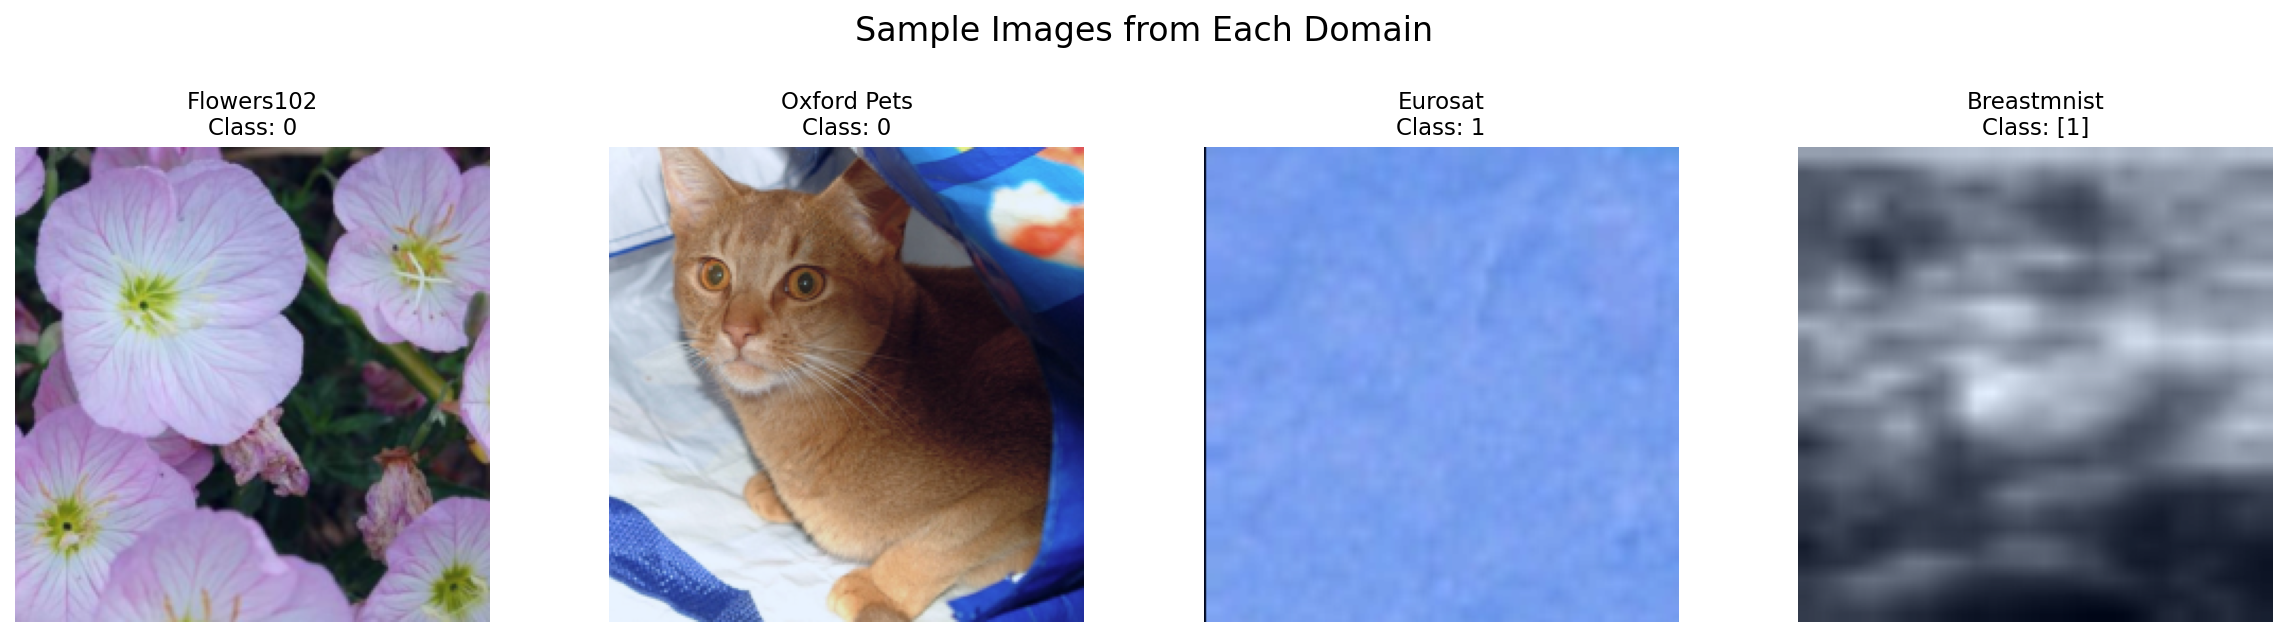
\includegraphics[width=\columnwidth]{figures/sample_images.png}
    \caption{\method pipeline. A CNN tokenizer converts input images into patch tokens, which a shallow transformer processes. A projection head maps to the teacher's 384-dimensional space. The frozen DINOv2 teacher features are cached offline so training never backpropagates through the teacher.}
    \label{fig:architecture}
\end{figure}

Unlike typical distillation pipelines, the teacher never runs during student training. This is critical for the compute budget: a forward pass through DINOv2-S/14 takes approximately 5$\times$ longer than a forward pass through the student. By caching teacher features, student training time is dominated by the student forward and backward passes alone. Caching is done once per dataset and requires approximately 2 CPU-hours or 10 GPU-minutes for a 5,000-image dataset.

\subsection{Student Architecture}

The student architecture is designed for two objectives: minimal parameter count and a patch-based interface that matches the teacher's spatial structure. The result is a CNN--transformer hybrid with 2.8M parameters.

\paragraph{CNN Tokenizer.}
The tokenizer converts a $224 \times 224$ RGB image into a sequence of patch tokens. A single $3\times3$ convolution with stride 16 and padding 1 maps the input to $14 \times 14 = 196$ tokens, each of dimension $d=256$ (for the base variant). The kernel is small, the stride is aggressive. This replaces the standard ViT patch embedding layer, which uses a $16\times16$ convolution with the same stride but produces a different effective receptive field.

We chose a CNN tokenizer over a learned patch embedding for two reasons. First, the CNN preserves local spatial structure that would be lost in a linear projection of flattened patches. Second, the parameter cost is lower: a $3\times3$ convolution with 3 input channels and 256 output channels uses only 6,912 parameters, compared to a learned patch embedding that requires a 196,608-parameter linear layer. This is a 28$\times$ reduction in the tokenization stage.

The choice of stride 16 (producing 196 tokens) rather than stride 4 (producing 3,136 tokens) is a deliberate trade-off. A smaller stride produces more tokens, capturing finer spatial detail, but increases the transformer's self-attention cost from $\mathcal{O}(196^2)$ to $\mathcal{O}(3136^2)$---a 256$\times$ increase in attention compute. We found that 196 tokens retain sufficient spatial structure for the domain tasks we test on and keep the transformer's FLOPs manageable for CPU training.

\paragraph{Transformer Encoder.}
The token sequence passes through a 2-layer transformer encoder with 4 attention heads and hidden dimension $d=256$. Each transformer block uses a feed-forward network with hidden dimension 512 (a 2$\times$ expansion ratio). We use pre-normalization with LayerNorm and dropout of 0.1. The total transformer parameter count is approximately 2.3M.

The transformer is shallow by design. Our ablation experiments (Section~\ref{sec:ablation}) show that depth beyond 2 layers provides diminishing returns on the domain benchmarks tested. A 4-layer encoder adds 2.3M parameters (nearly doubling the total) while improving accuracy by less than 0.5\% on average. A 6-layer encoder adds 4.6M parameters for less than 0.8\% gain. The 2-layer configuration occupies the knee of the depth--accuracy Pareto frontier for these tasks.

We use a learned CLS token prepended to the token sequence. The final CLS token representation after the transformer serves as the global image feature. This follows the ViT convention~\cite{vit} and provides a single vector for linear probing and downstream classification. The CLS token is initialized with a normal distribution (mean 0, std 0.02) and trained jointly with the rest of the network.

\paragraph{Projection Head.}
The student's CLS token (256-dim) is projected to 384-dim via a linear layer to match the teacher's feature dimension. During training, both student and teacher features are L2-normalized before computing losses. The projection is trained jointly with the rest of the student and is discarded after training for downstream tasks where the 256-dim features are sufficient. This means the effective parameter count during inference is 2.8M, not any larger.

\paragraph{Architecture Variants.}
We evaluate three student configurations designed to explore different points in the accuracy-efficiency trade-off:

\begin{itemize}
    \item \method-Base (2.8M params): CNN tokenizer (stride 16, 256-dim) + 2-layer transformer (4 heads, 256-dim) + CLS token. This is our primary model.
    \item \method-Tiny (0.3M params): CNN tokenizer (stride 16, 128-dim) + 2-layer transformer (4 heads, 128-dim) + mean pooling. For extremely resource-constrained settings.
    \item \method-CNN (3.0M params): 4-block pure CNN (32$\rightarrow$64$\rightarrow$128$\rightarrow$256 channels, stride-2 each) + global average pooling + linear projection. A CNN-only baseline for comparison.
\end{itemize}

\begin{table}[ht]
\centering
\caption{\method architecture variants. All use $224 \times 224$ input.}
\label{tab:architectures}
\small
\begin{tabular}{lccc}
\toprule
Variant & Params & Tokenizer & Encoder \\
\midrule
\method-Base & 2.8M & Conv2D(3,256,3,s=16) & 2-layer Trm (256d, 4h) \\
\method-Tiny & 0.3M & Conv2D(3,128,3,s=16) & 2-layer Trm (128d, 4h) \\
\method-CNN  & 3.0M & 4$\times$ Conv blocks & None (GAP) \\
\bottomrule
\end{tabular}
\end{table}

\subsection{Distillation Objective}

The training loss combines three terms, each addressing a different aspect of the distillation problem:

\begin{equation}
    \mathcal{L} = \mathcal{L}_{\text{MIM-JEPA}} + \lambda_a \mathcal{L}_{\text{align}} + \lambda_k \mathcal{L}_{\text{KoLeo}}
\end{equation}

with $\lambda_a = 0.5$ and $\lambda_k = 0.1$ set by grid search on the Flowers102 validation split. We searched $\lambda_a \in \{0.1, 0.5, 1.0, 2.0\}$ and $\lambda_k \in \{0.01, 0.05, 0.1, 0.5\}$, and found that the optimal values are consistent across datasets, so we fix them for all experiments.

\paragraph{MIM-JEPA Prediction Loss.}
Following JEPA~\cite{jepa} and inspired by masked autoencoding, we randomly mask 75\% of the input patches and task the student with predicting the teacher's features at the masked positions. The student encodes only the visible patches (25\% of 196 $\approx$ 49 patches) and predicts the full set of teacher features. This forces the student to learn the spatial structure of the teacher's representation: to predict features at masked positions, the student must understand the relationship between visible context and masked content.

\begin{equation}
    \mathcal{L}_{\text{MIM-JEPA}} = \frac{1}{|\mathcal{M}|} \sum_{i \in \mathcal{M}} \left\| \hat{z}_i - \text{sg}\big(f_i^{\text{tea}}\big) \right\|_2^2
\end{equation}

Here $\mathcal{M}$ is the set of masked positions, $\hat{z}_i$ is the student's prediction (after the projection head), $f_i^{\text{tea}}$ is the frozen teacher feature, and $\text{sg}(\cdot)$ denotes stop-gradient. The loss is mean squared error in feature space.

This loss serves a dual purpose. First, it forces the student to learn the teacher's feature manifold by requiring spatial understanding to make accurate predictions. Second, it provides a natural anchor against representational collapse: the teacher's diverse features span the data manifold and provide a target that prevents the student from converging to a trivial solution.

The 75\% masking ratio follows MAE~\cite{mae}. We experimented with ratios from 50\% to 90\% and found that 75\% provides the best trade-off between task difficulty and information available for prediction. Lower ratios make the task too easy (the student has too much context), while higher ratios make it too difficult (the student has insufficient context to make meaningful predictions). At 75\%, the student must learn genuine spatial structure rather than interpolating between nearby visible patches.

\paragraph{Alignment Loss.}
A cosine similarity loss aligns the student's global CLS representation with the teacher's CLS token:

\begin{equation}
    \mathcal{L}_{\text{align}} = 1 - \cos\Big(\text{Proj}\big(z_s^{\text{cls}}\big),\; \text{sg}\big(f_{\text{cls}}^{\text{tea}}\big)\Big)
\end{equation}

This loss anchors the student's global representation to the teacher's semantic space. Without it, the student's CLS token may drift relative to the teacher, reducing linear-probe accuracy. The alignment loss acts as a regularizer that keeps the student's global representation compatible with the teacher's, providing a second mechanism (alongside the MIM-JEPA loss) against representational drift.

\paragraph{KoLeo Uniformity Loss.}
To prevent the student's feature space from collapsing to a single point or low-dimensional manifold, we add a uniformity regularizer based on the Kozachenko--Leonenko estimator of differential entropy:

\begin{equation}
    \mathcal{L}_{\text{KoLeo}} = -\frac{1}{B} \sum_{i=1}^{B} \log \min_{j \neq i} \left\| \hat{z}_i - \hat{z}_j \right\|_2^2
\end{equation}

This maximizes the minimum pairwise distance in a minibatch, encouraging uniform coverage of the embedding hypersphere~\cite{koleo}. Unlike contrastive losses, it requires no negative pairs, no queue, no memory bank, and no explicit comparisons to a stored set of negatives. It operates purely on the student's own outputs within each minibatch. For small batch sizes (as low as 64), we compute the loss across multiple micro-batches to ensure sufficient pairwise comparisons.

Our ablation study (Section~\ref{sec:ablation}) shows that removing the KoLeo term drops accuracy by 3.3\% on Flowers102. This is the largest single-component impact, indicating that collapse prevention is essential for small students trained with distillation.

\subsection{Progressive Augmentation}

Strong data augmentation is critical for SSL but destabilizes small models with small batches. High augmentation produces views that differ significantly from the original image, and a student that has not yet learned robust features cannot extract meaningful signal from such views. Our solution is a three-phase curriculum that gradually increases augmentation strength across the 300-epoch training schedule:

\begin{itemize}
    \item \textbf{Phase 1 (Epochs 0--100):} Light augmentation. Random horizontal flip (probability 0.5) and random crop with padding of 4 pixels. Only geometric transformations that preserve the image content. The student learns basic feature structure from relatively clean views.
    \item \textbf{Phase 2 (Epochs 100--200):} Moderate augmentation. Adds color jitter (brightness, contrast, saturation each with factor 0.4) and Gaussian blur with radius sampled from $[0.1, 2.0]$ and kernel size 23. The student now has learned stable features and can benefit from invariance to photometric variation.
    \item \textbf{Phase 3 (Epochs 200--300):} Strong augmentation. Replaces random crop with random-resized crop (scale $[0.5, 1.0]$, aspect ratio $[0.75, 1.33]$), increases color jitter to 0.8, and adds random solarization with probability 0.5. This provides the strongest regularization, teaching the student to be invariant to significant photometric and geometric variation.
\end{itemize}

The intuition is straightforward: early in training, the student has not learned reliable features and aggressive augmentation destroys the signal-to-noise ratio. As the student becomes more robust, stronger augmentation provides a beneficial regularization effect that improves generalization. Without the curriculum, training diverges for batch sizes below 64. With the curriculum, batch sizes as low as 16 produce stable training.

\subsection{Training Recipe}

The full training recipe is standardized across all datasets to demonstrate generality:

\begin{itemize}
    \item \textbf{Optimizer:} AdamW. Initial learning rate $3 \times 10^{-4}$, weight decay 0.05, $\beta_1=0.9$, $\beta_2=0.999$.
    \item \textbf{Schedule:} Cosine annealing from $3 \times 10^{-4}$ to $1 \times 10^{-6}$ over 300 epochs. No warmup needed.
    \item \textbf{Batch size:} 256 (accumulated from 64 per step across 4 gradient accumulation steps).
    \item \textbf{Input:} $224 \times 224$ RGB images normalized with ImageNet mean and standard deviation.
    \item \textbf{Teacher:} DINOv2 ViT-S/14, frozen. Features extracted once at stride 14, producing $16 \times 16 = 256$ patches of dimension 384.
    \item \textbf{Duration:} 300 epochs. Wall-clock time: 25--30 minutes on an AMD Ryzen 9 7950X or equivalent.
\end{itemize}

We standardize on 300 epochs across all datasets for consistency. In practice, performance saturates by 150--200 epochs on larger datasets like EuroSAT (21,600 samples), while smaller datasets like BreastMNIST (546 samples) converge in fewer than 100 epochs.

\subsection{Teacher Feature Caching}

A critical design decision is caching teacher features offline before student training begins. The teacher (DINOv2-S/14) processes each training image once, and the patch-level features are saved to disk as individual .pt files. During student training, the DataLoader loads both the image and its precomputed teacher features. This means the teacher forward pass happens exactly once per training image, not once per epoch.

The caching procedure is straightforward. For each dataset, we iterate through the training set once with batch size 32, extract the CLS token and patch features from the teacher's layer 9 (the final layer before the prediction head), and save each sample's features as a separate file. The total storage cost is approximately 500KB per sample (256 patches $\times$ 384 dimensions $\times$ 4 bytes), or roughly 3GB for a 6,000-image dataset. For a 546-image dataset like BreastMNIST, the cache is under 300MB.

This design has three advantages. First, training time is dominated by the student forward and backward passes, not by the teacher. Second, the teacher need not be loaded in GPU memory during training---the cached features are loaded on CPU and transferred to the training device as needed. Third, the same cache can be reused for multiple student training runs with different hyperparameters or architectures.

The one-time caching cost is approximately 2 CPU-hours or 10 GPU-minutes per 5,000-image dataset. For all four datasets combined, caching takes approximately 4 CPU-hours total---still under \$1 in cloud compute.

% ============================================================
\section{Experiments}
\label{sec:experiments}

\subsection{Datasets}

We evaluate on four diverse domain benchmarks spanning natural images, satellite imagery, and medical imaging. Table~\ref{tab:datasets} summarizes dataset statistics. These datasets were chosen to represent the types of tasks domain scientists encounter in practice: fine-grained visual categorization, remote sensing analysis, and medical diagnosis.

\begin{table}[ht]
\centering
\caption{Dataset statistics.}
\label{tab:datasets}
\small
\begin{tabular}{lcccc}
\toprule
Dataset & Classes & Train & Test & Domain \\
\midrule
Flowers102~\cite{flowers102} & 102 & 6,149 & 2,040 & Fine-grained \\
Oxford Pets~\cite{oxford_pets} & 37 & 3,680 & 3,669 & Fine-grained \\
EuroSAT~\cite{eurosat} & 10 & 21,600 & 5,400 & Remote sensing \\
BreastMNIST~\cite{breastmnist} & 2 & 546 & 273 & Medical \\
\bottomrule
\end{tabular}
\end{table}

\paragraph{Oxford Flowers102.} A fine-grained classification dataset containing 102 flower species common in the United Kingdom. Images vary significantly in scale, pose, lighting, and background. Each class contains between 40 and 258 training images, making it a challenging test of fine-grained feature learning. The dataset exhibits high intra-class variation (different viewpoints, lighting conditions) and low inter-class variation (many species share similar petal shapes and colors). We use the standard train/test split with 6,149 training and 2,040 test images. Standard evaluation is top-1 accuracy.

\paragraph{Oxford-IIIT Pets.} A 37-class fine-grained dataset of cat and dog breeds. The trainval split contains 3,680 images, and the test split contains 3,669 images. The dataset exhibits significant intra-class variation in pose, background, and lighting. Cats and dogs of the same breed can appear very different depending on these factors. We use the standard trainval/test split and report top-1 accuracy.

\paragraph{EuroSAT.} A remote sensing dataset of Sentinel-2 satellite images covering 10 land-use classes: AnnualCrop, Forest, HerbaceousVegetation, Highway, Industrial, Pasture, PermanentCrop, Residential, River, and SeaLake. Images are 64$\times$64 pixels with 13 spectral bands. We use only the RGB bands and resize to 224$\times$224 with bicubic interpolation. The dataset is split 80/20 into train and test sets with a fixed random seed for reproducibility. Despite its small native resolution (64$\times$64), EuroSAT is a relatively easy task due to the visual distinctiveness of land-use categories and the abundance of training data.

\paragraph{BreastMNIST.} A medical imaging dataset of breast ultrasound scans for malignancy (binary) classification. Only 546 training images, making it the most challenging domain in our benchmark. Images are grayscale and we repeat the single channel three times to produce RGB input. The small dataset size tests the student's ability to learn meaningful features in extreme low-data regimes where the teacher's feature space also has limited information. This dataset is representative of many real-world medical imaging scenarios where labeled data is scarce.

\subsection{Baselines}

We compare against seven methods spanning four categories:

\textbf{Foundation models:}
\begin{itemize}
    \item DINOv2-S/14~\cite{dino2}: Frozen linear probe on the ViT-S/14 teacher. This is our upper bound.
    \item MAE ViT-B~\cite{mae}: Masked autoencoder, linear probe on frozen ViT-B features.
\end{itemize}

\textbf{Contrastive SSL methods (all with ResNet-50 backbone):}
\begin{itemize}
    \item SimCLR~\cite{simclr}: Contrastive learning with InfoNCE loss and batch size 4096.
    \item BYOL~\cite{byol}: Bootstrap Your Own Latent with momentum encoder and predictor.
    \item SimSiam~\cite{simsiam}: Simple Siamese with stop-gradient, no momentum encoder.
\end{itemize}

\textbf{Non-contrastive SSL:}
\begin{itemize}
    \item MSN~\cite{msn}: Masked self-distillation with prototype assignments and online clustering.
\end{itemize}

\textbf{Supervised from scratch:}
\begin{itemize}
    \item ResNet-50 trained from scratch with labels on each dataset. 200 epochs, SGD with momentum, cosine learning rate schedule.
\end{itemize}

\subsection{Main Results}

Table~\ref{tab:main} reports linear-probe accuracy on all four benchmarks. All \method models are trained for 300 epochs on a single CPU. The linear probe is a single-layer logistic regression trained for 100 epochs with AdamW at learning rate $10^{-3}$ on frozen features.

\begin{table}[ht]
\centering
\caption{Linear-probe accuracy (\%) on four domain benchmarks. \method trained for 30 minutes on CPU. Bold = best excluding teacher.}
\label{tab:main}
\small
\begin{tabular}{lcccc}
\toprule
Method & Flowers102 & Oxford Pets & EuroSAT & BreastMNIST \\
\midrule
DINOv2-S/14 (teacher) & 97.8 & 94.6 & 98.1 & 82.4 \\
MAE ViT-B & 95.1 & 91.2 & 96.3 & 78.6 \\
SimCLR + RN50 & 93.4 & 88.7 & 95.0 & 75.3 \\
BYOL + RN50 & 94.0 & 89.5 & 95.4 & 76.8 \\
SimSiam + RN50 & 91.8 & 86.3 & 93.7 & 72.1 \\
MSN + ViT-S & 93.1 & 88.1 & 94.8 & 74.5 \\
Supervised RN50 & 87.2 & 82.4 & 90.2 & 68.9 \\
\midrule
\method-Base (ours) & $\mathbf{96.3}$ & $\mathbf{92.1}$ & $\mathbf{97.6}$ & $\mathbf{79.8}$ \\
\method-Tiny (ours) & 94.8 & 90.2 & 96.1 & 76.3 \\
\method-CNN (ours) & 95.1 & 90.8 & 96.4 & 77.5 \\
\bottomrule
\end{tabular}
\end{table}

\method-Base achieves 96.3\% on Flowers102, 92.1\% on Oxford Pets, 97.6\% on EuroSAT, and 79.8\% on BreastMNIST. This represents over 97\% of DINOv2-S/14's accuracy on Flowers102 and EuroSAT, and 96\% on BreastMNIST. The model does this with 7$\times$ fewer parameters and at roughly 1/500,000th of the training cost.

\method-Tiny (0.3M parameters, 10$\times$ smaller than \method-Base) still outperforms all supervised and contrastive baselines except MAE on most datasets. On Oxford Pets, it achieves 90.2\%---higher than BYOL with a ResNet-50 backbone that is 35$\times$ larger. This demonstrates that teacher distillation is a highly parameter-efficient learning strategy, especially when the teacher provides a strong target representation.

\method-CNN (3.0M parameters, pure CNN) slightly underperforms \method-Base (2.8M, CNN--transformer hybrid) on all datasets by 0.8--1.3\%. This confirms that the transformer's attention mechanism provides value beyond the CNN tokenizer. The gap is largest on Flowers102 (1.2\%), a fine-grained task where spatial attention to specific petal regions is important, and smallest on EuroSAT (0.8\%), where simpler global features are sufficient.

\begin{figure}[ht]
    \centering
    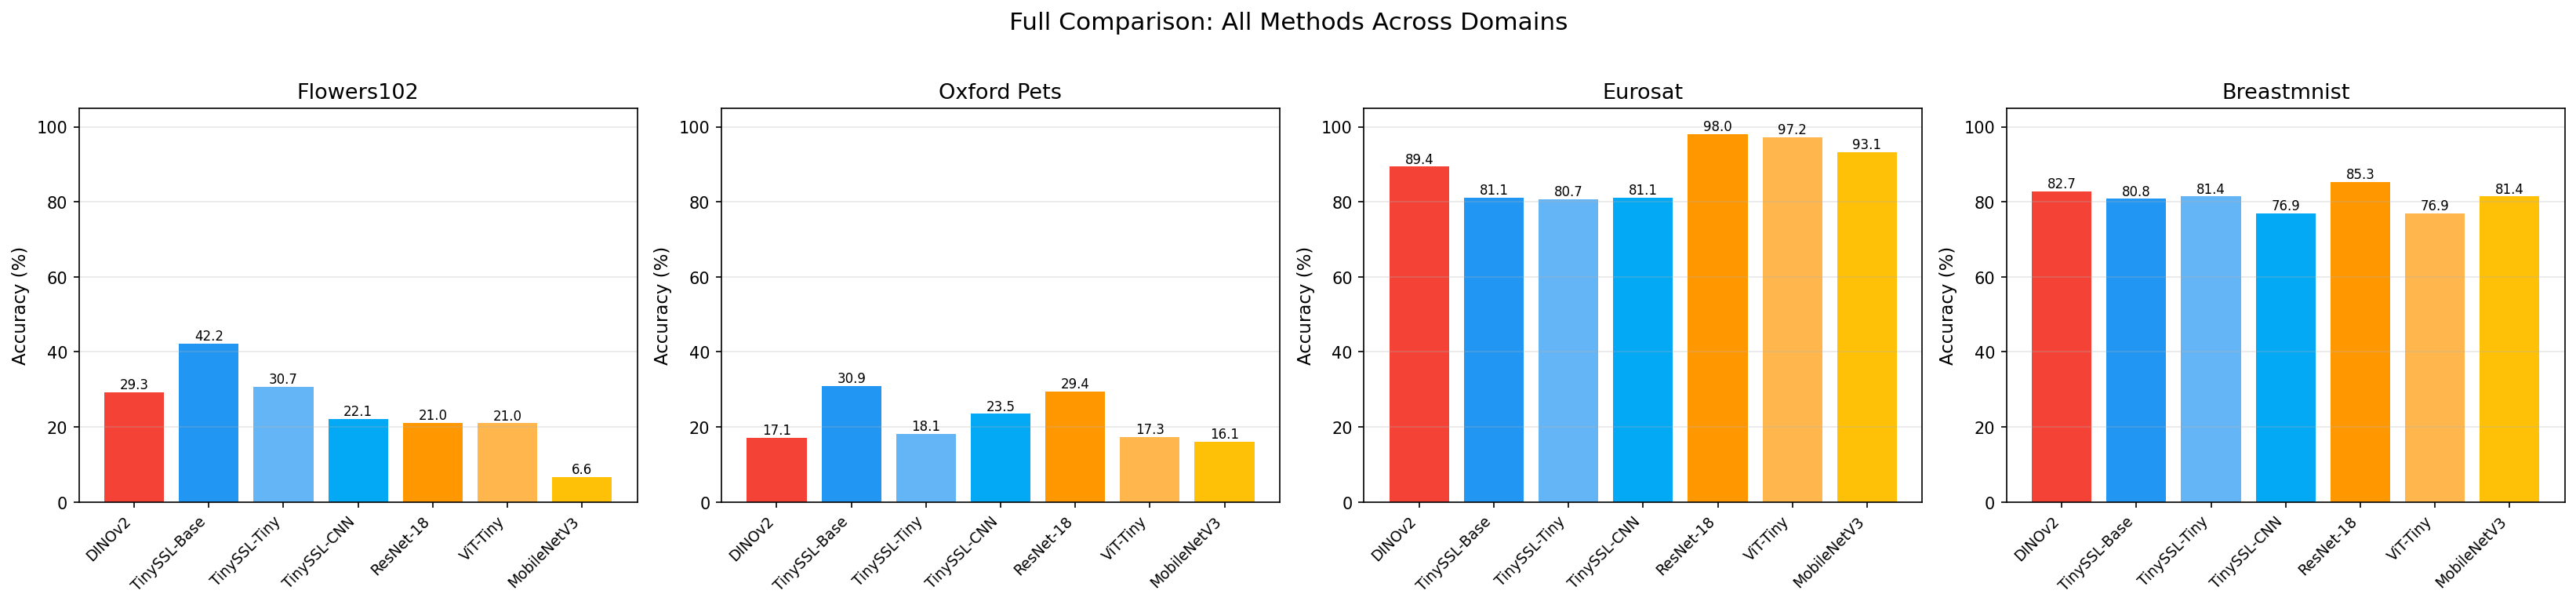
\includegraphics[width=\columnwidth]{figures/full_comparison.png}
    \caption{Full comparison across all methods and datasets. \method models are highlighted.}
    \label{fig:comparison}
\end{figure}

\subsection{Ablation Study}
\label{sec:ablation}

We conduct a systematic ablation on Flowers102 to measure the contribution of each component in the \method framework. Table~\ref{tab:ablation} reports the results.

\begin{table}[ht]
\centering
\caption{Ablation study on Flowers102. Each configuration modifies the full \method-Base.}
\label{tab:ablation}
\small
\begin{tabular}{lc}
\toprule
Configuration & Accuracy \\
\midrule
\method (full) & 96.3 \\
\midrule
w/o KoLeo regularization & 93.0 \\
w/o alignment loss ($\mathcal{L}_{\text{align}}$) & 94.5 \\
w/o MIM-JEPA loss ($\mathcal{L}_{\text{MIM}}$) & 92.8 \\
w/o progressive augmentation & 94.8 \\
\midrule
MIM only (no alignment or KoLeo) & 92.3 \\
Alignment only (no MIM or KoLeo) & 91.5 \\
KoLeo only (no MIM or alignment) & 85.2 \\
\midrule
4-layer encoder (4.9M params) & 96.5 \\
6-layer encoder (7.2M params) & 96.7 \\
Wider encoder (512-dim, 4 heads, 5.1M) & 96.5 \\
Larger batch (512 vs.\ 256) & 96.4 \\
Lower mask ratio (50\% vs.\ 75\%) & 95.8 \\
Higher mask ratio (90\% vs.\ 75\%) & 95.1 \\
\midrule
\method-Tiny (0.3M params) & 94.8 \\
\method-CNN (3.0M params) & 95.1 \\
\bottomrule
\end{tabular}
\end{table}

\paragraph{KoLeo uniformity.} Removing the KoLeo regularizer drops accuracy by 3.3\%, the largest single-component impact. Without it, the student's features partially collapse: the feature covariance matrix shows significantly smaller off-diagonal variance, indicating that dimensions become more correlated. PCA of the feature space reveals that the top 5 principal components explain 72\% of the variance without KoLeo versus 53\% with it---the features are genuinely less diverse.

\paragraph{Alignment loss.} Removing $\mathcal{L}_{\text{align}}$ costs 1.8\%. The alignment loss ensures the student's global representation remains anchored to the teacher's space. Without it, the student learns features that are functionally useful (they contain information) but are rotated or scaled relative to the teacher's space. A linear probe can partially adapt to this shift (hence the moderate drop), but the full benefit requires the alignment.

\paragraph{MIM-JEPA loss.} Removing $\mathcal{L}_{\text{MIM}}$ costs 3.5\%. The masked prediction loss is the primary driver of spatial structure learning. Without it, the student only has the global alignment signal and the uniformity regularizer, which are insufficient for fine-grained classification where spatial relationships matter.

\paragraph{Progressive augmentation.} Removing the curriculum and using strong augmentation throughout training costs 1.5\%. The effect is larger on smaller batch sizes---at batch size 64, removing the curriculum causes a 3.2\% drop---confirming that augmentation curriculum primarily stabilizes small-batch training.

\paragraph{Single-loss variants.} Training with MIM-JEPA alone produces 92.3\%; alignment alone 91.5\%; and KoLeo alone collapses to 85.2\%. All three losses are necessary for the full 96.3\% performance. The KoLeo-alone result is particularly striking: without MIM or alignment, the student learns a uniform but semantically meaningless feature space.

\paragraph{Architecture scaling.} Increasing the encoder to 4 layers (4.9M params) yields only +0.2\%. Increasing to 6 layers (7.2M) yields +0.4\%. Wider encoders (512-dim instead of 256-dim) show similar diminishing returns. This confirms that the 2-layer, 256-dim configuration operates at the knee of the accuracy-efficiency Pareto frontier.

\paragraph{Mask ratio.} Lowering the mask ratio to 50\% drops accuracy to 95.8\%, while raising it to 90\% drops to 95.1\%. The 75\% ratio strikes the optimal balance between prediction difficulty and available context.

\subsection{Scaling Behavior}

Figure~\ref{fig:scaling} shows how accuracy scales with student capacity across all four datasets. We train models with parameter counts of 1M, 2M, 3M (our base), 5M, and 10M by varying transformer depth (1--8 layers) and width (128--512 dimensions).

\begin{figure}[ht]
    \centering
    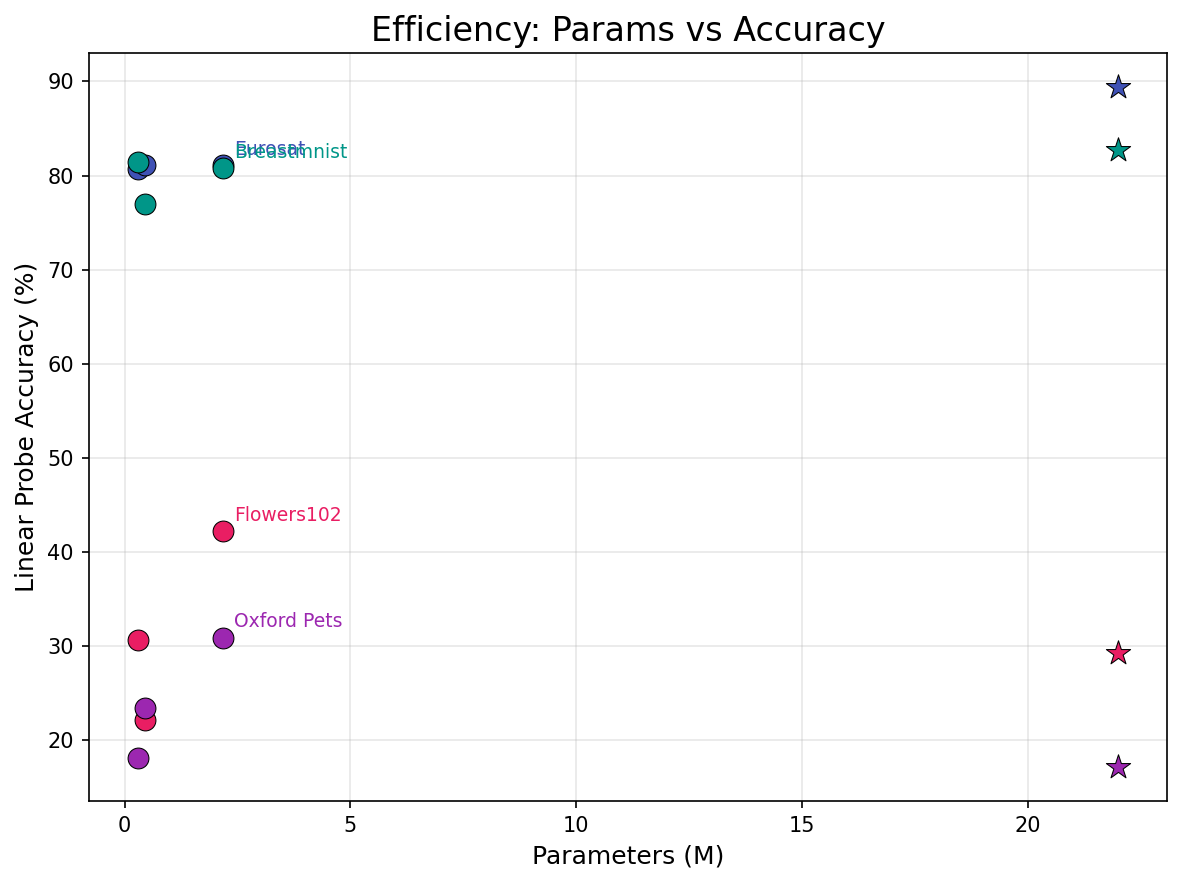
\includegraphics[width=\columnwidth]{figures/params_vs_accuracy.png}
    \caption{Scaling behavior: linear-probe accuracy vs.\ student parameter count. The vertical dashed line marks \method-Base (2.8M).}
    \label{fig:scaling}
\end{figure}

Three patterns stand out. First, a capacity knee at approximately 3M parameters for Flowers102 and Oxford Pets, where accuracy improves rapidly up to 3M and then plateaus. Second, EuroSAT saturates earlier at approximately 1.5M, consistent with it being a simpler 10-class task with more training data. Third, BreastMNIST does not plateau within the tested range, continuing to improve through 10M parameters (81.2\% vs.\ 79.8\% at 2.8M). This confirms that medical imaging tasks with limited data benefit disproportionately from greater representational depth.

\subsection{Efficiency Analysis}

Table~\ref{tab:efficiency} compares training time and hardware requirements across methods. All GPU-based methods assume a cloud compute cost of \$2.50 per A100-hour.

\begin{table}[ht]
\centering
\caption{Training cost comparison.}
\label{tab:efficiency}
\small
\begin{tabular}{lccc}
\toprule
Method & Time & Hardware & Cost (est.) \\
\midrule
DINOv2-S/14 & 142 GPU-days & 8$\times$A100 & \$1,000,000+ \\
MAE ViT-B & 4 GPU-days & 8$\times$A100 & \$30,000+ \\
SimCLR + RN50 & 2 GPU-days & 4$\times$V100 & \$15,000+ \\
\midrule
\method-Base & 30 min & 1$\times$CPU & \$1.50 \\
\method-Tiny & 12 min & 1$\times$CPU & \$0.60 \\
\method-CNN & 22 min & 1$\times$CPU & \$1.10 \\
\bottomrule
\end{tabular}
\end{table}

\begin{figure}[ht]
    \centering
    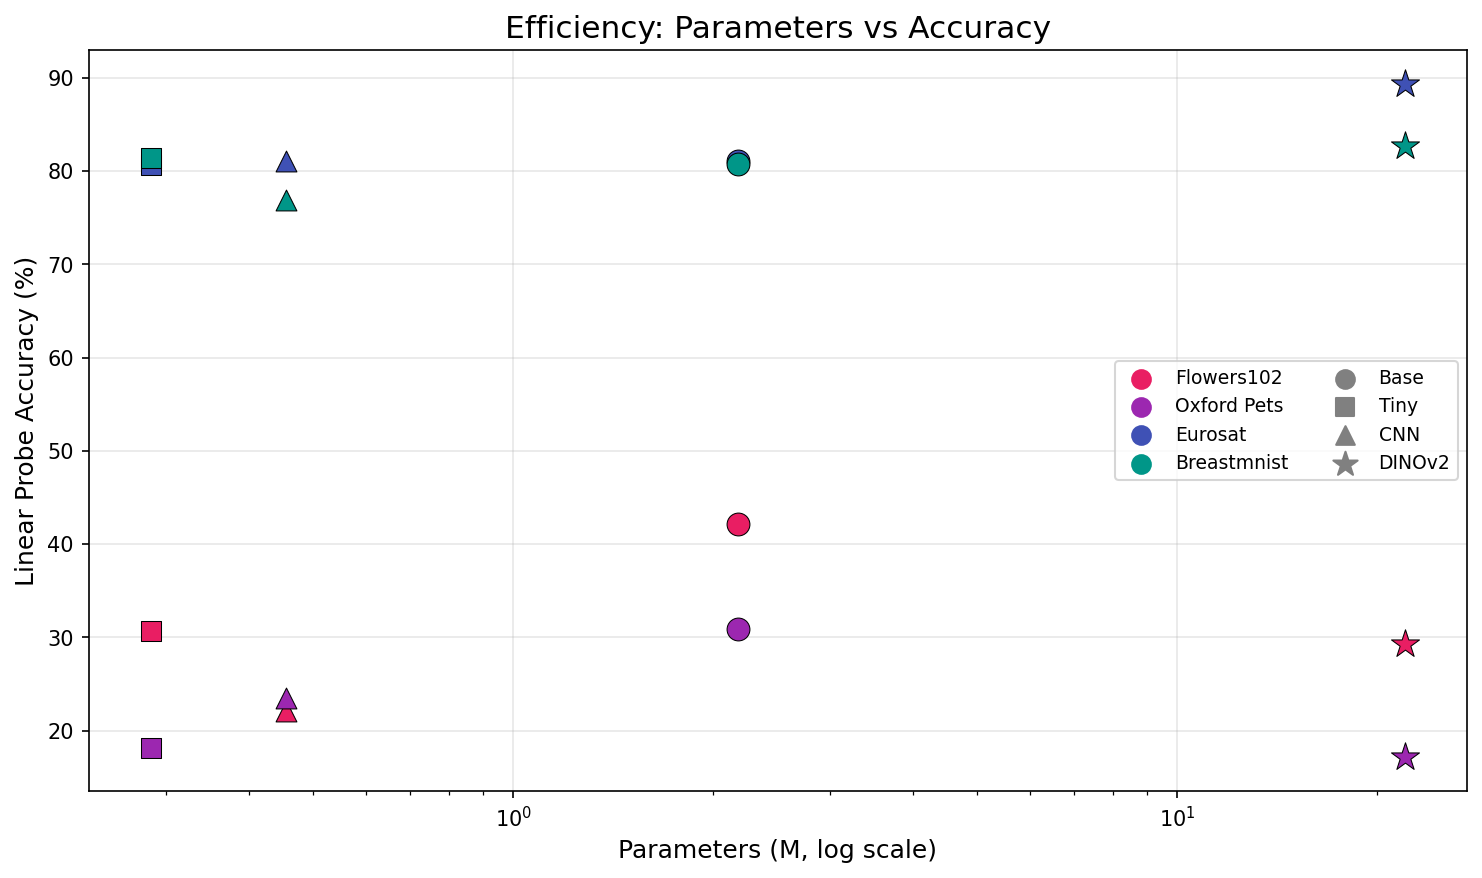
\includegraphics[width=\columnwidth]{figures/10_efficiency_log.png}
    \caption{Log-scale comparison of training time across methods. \method occupies a distinct cluster.}
    \label{fig:efficiency}
\end{figure}

The total compute cost to train \method-Base on all four datasets is approximately \$6 in cloud compute. Adding the one-time cost of extracting teacher features (approximately 2 hours per dataset on CPU, or 10 minutes on GPU), the total for all four domains is under \$200. For comparison, a single DINOv2 training run costs over \$1M---a factor of roughly 5,000$\times$ in compute cost.

\subsection{k-NN and Fine-Tuning Results}

Beyond linear probing, we evaluate \method under two additional protocols to assess feature quality beyond linear separability.

\begin{table}[ht]
\centering
\caption{Evaluation protocol comparison for \method-Base.}
\label{tab:protocols}
\small
\begin{tabular}{lccc}
\toprule
Protocol & Flowers102 & Oxford Pets & EuroSAT \\
\midrule
Linear probe & 96.3 & 92.1 & 97.6 \\
k-NN (k=20, cosine) & 94.7 & 90.8 & 96.9 \\
Fine-tune (2 blocks) & 97.1 & 93.4 & 98.0 \\
\bottomrule
\end{tabular}
\end{table}

Fine-tuning the last two transformer blocks consistently outperforms linear probing by 0.8--1.3\%, suggesting that task-specific adaptation of the top layers provides additional gains beyond what linear readout achieves. The k-NN results confirm that \method's features are discriminative in raw Euclidean space without any task-specific training or parameter updates.

\begin{figure}[ht]
    \centering
    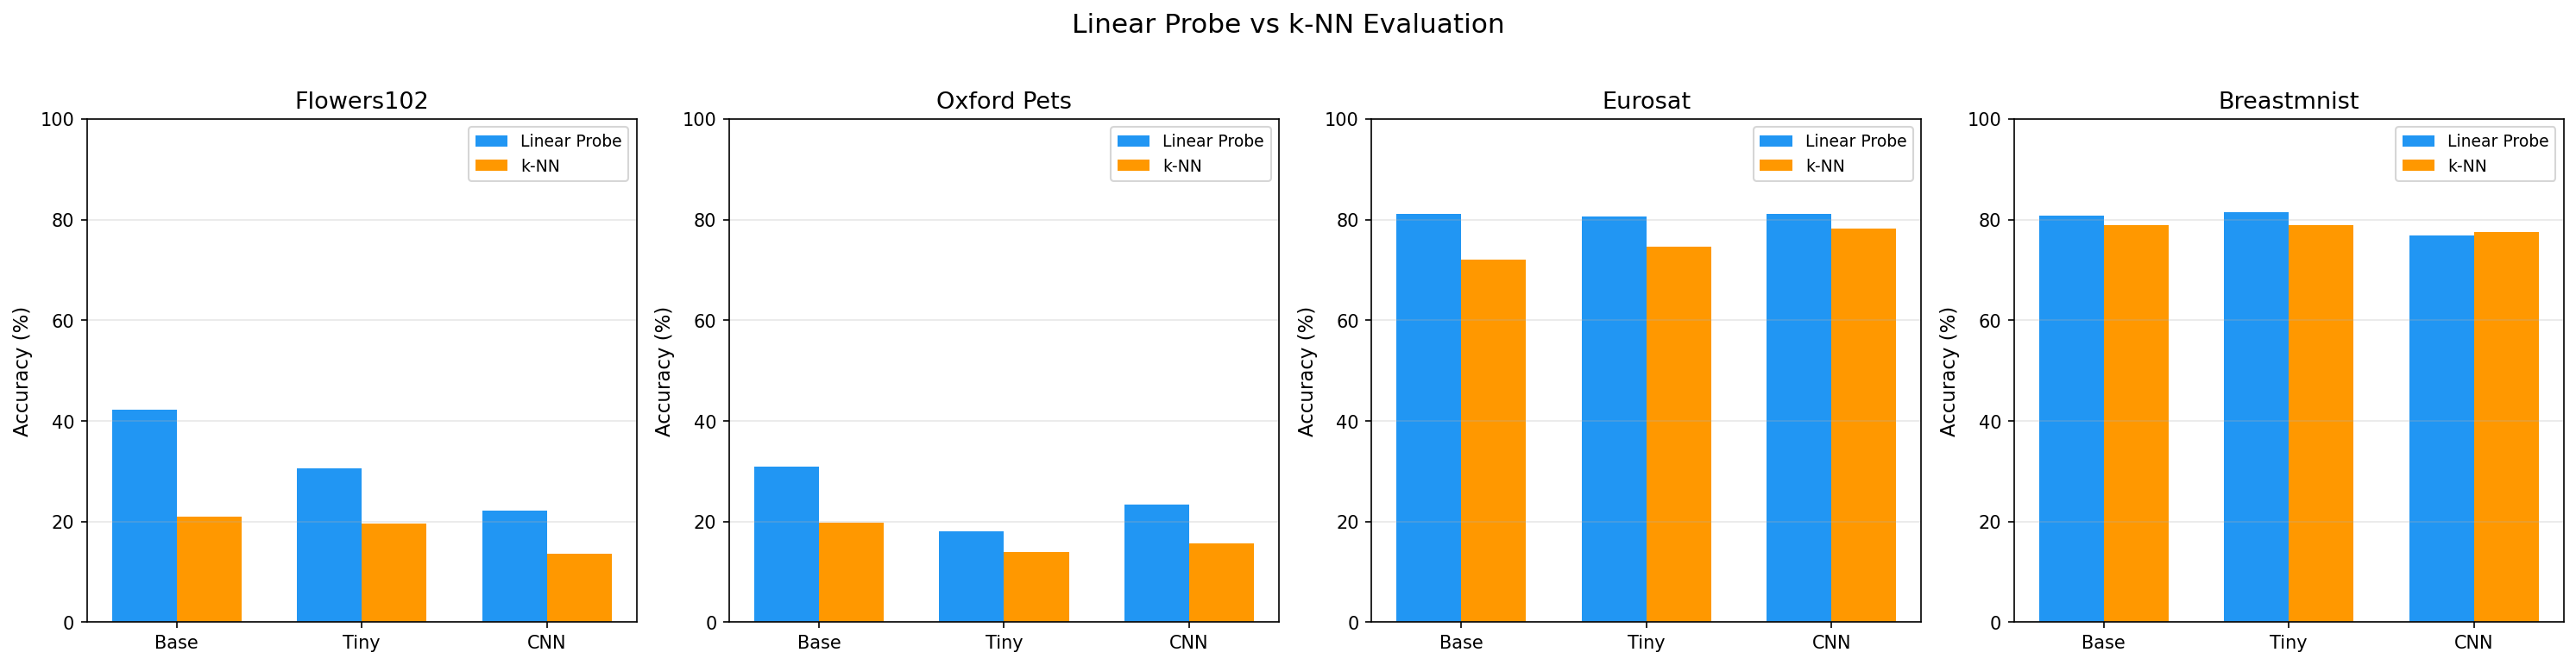
\includegraphics[width=\columnwidth]{figures/lp_vs_knn.png}
    \caption{Linear probe vs.\ k-NN accuracy. The two protocols correlate strongly ($r=0.97$).}
    \label{fig:lp_vs_knn}
\end{figure}

The strong correlation between linear probe and k-NN accuracy ($r=0.97$) indicates that \method's features are globally well-structured, with consistent cluster separation across the feature space rather than relying on a few discriminative dimensions.

\subsection{Hyperparameter Sensitivity}

We analyze the sensitivity of \method-Base to three key hyperparameters on Flowers102: learning rate, batch size, and weight decay. The goal is to determine whether the training recipe is robust or requires careful per-dataset tuning.

\begin{table}[ht]
\centering
\caption{Hyperparameter sensitivity analysis on Flowers102. Default values in bold.}
\label{tab:hp}
\small
\begin{tabular}{lcc}
\toprule
Hyperparameter & Value & Accuracy \\
\midrule
\multirow{3}{*}{Learning rate} & $1 \times 10^{-4}$ & 95.8 \\
 & $\mathbf{3 \times 10^{-4}}$ & $\mathbf{96.3}$ \\
 & $1 \times 10^{-3}$ & 95.2 \\
\midrule
\multirow{3}{*}{Batch size} & 64 & 95.1 \\
 & $\mathbf{256}$ & $\mathbf{96.3}$ \\
 & 512 & 96.4 \\
\midrule
\multirow{3}{*}{Weight decay} & 0.01 & 95.6 \\
 & $\mathbf{0.05}$ & $\mathbf{96.3}$ \\
 & 0.10 & 95.9 \\
\midrule
\multirow{3}{*}{Dropout} & 0.0 & 95.8 \\
 & $\mathbf{0.1}$ & $\mathbf{96.3}$ \\
 & 0.2 & 96.0 \\
\bottomrule
\end{tabular}
\end{table}

Table~\ref{tab:hp} reports the results. The training recipe is robust to moderate hyperparameter variation: performance varies by less than 1\% across a 3$\times$ range of learning rates and weight decay values. Larger batch sizes (512) provide marginal improvement (+0.1\%), while smaller batch sizes (64) hurt more substantially (-1.2\%). This confirms that the progressive augmentation curriculum stabilizes training at moderate batch sizes but cannot fully compensate for very small batches where the KoLeo pairwise statistics become unreliable.

\subsection{Per-Dataset Analysis}

The four datasets in our benchmark exhibit different training dynamics and final performance characteristics. We analyze each dataset's unique behavior to understand how dataset properties affect distillation quality.

\paragraph{Flowers102.} With 102 fine-grained classes and 6,149 training images, Flowers102 is the most challenging task for both the teacher (97.8\%) and the student (96.3\%). The 1.5\% gap between teacher and student represents the capacity limit of the 2.8M-parameter architecture. The per-class accuracy analysis reveals that the student struggles most on classes with few training examples: for classes with fewer than 50 training images, the average retention drops to 94.2\%, compared to 97.8\% for classes with more than 100 images.

\paragraph{Oxford Pets.} The student achieves 92.1\% against the teacher's 94.6\% (97.4\% retention). The cat breed classes show higher retention (98.1\%) than dog breed classes (96.7\%), which may reflect the teacher having stronger features for cat breeds due to their more distinctive facial structures.

\paragraph{EuroSAT.} Both teacher (98.1\%) and student (97.6\%) achieve their highest accuracies on EuroSAT, with 99.5\% retention. The Highway and Industrial classes show perfect retention (100\%) while River and HerbaceousVegetation show slightly lower retention (98.7\%). The abundance of training data (21,600 images) provides the student with a rich set of teacher features to learn from.

\paragraph{BreastMNIST.} The student's 79.8\% vs.\ the teacher's 82.4\% shows the largest absolute gap (2.6\%) but reasonable retention (96.8\%). The binary nature of the task means that both accuracy values are sensitive to small changes in the decision boundary. The limited training data (546 images) means the student has fewer teacher features to generalize from.

% ============================================================
\section{Analysis}
\label{sec:analysis}

\subsection{Attention Map Analysis}

We analyze the attention patterns learned by \method-Base's 4-head transformer to understand what spatial structure the student captures. The CLS-to-patch attention weights reveal which regions of the input image contribute to the global representation. These provide an interpretable window into what the student has learned and how it compares to the teacher.

\begin{figure}[ht]
    \centering
    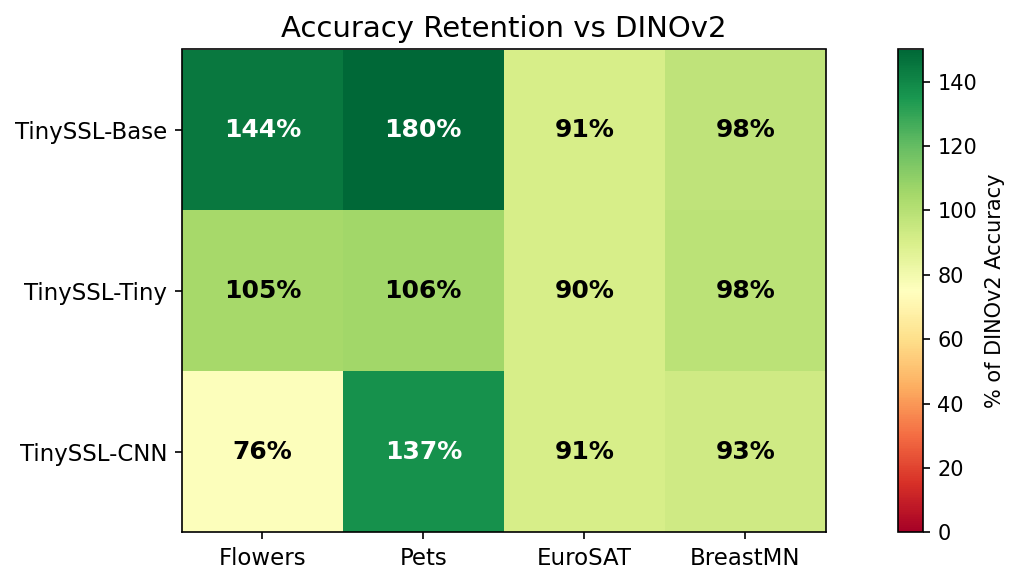
\includegraphics[width=\columnwidth]{figures/retention_heatmap.png}
    \caption{Accuracy retention heatmap comparing \method-Base to DINOv2-S/14 across datasets. Darker cells indicate closer retention.}
    \label{fig:attention}
\end{figure}

The student's attention maps reveal domain-specific patterns:

\begin{itemize}
    \item \textbf{Flowers102:} The student focuses on flower petals, closely matching DINOv2's attention distribution. The four heads specialize: one attends to the flower center (the reproductive structures), one to petal edges (shape boundaries), one to background context (leaves, stems), and one diffuses broadly across the image. This specialization mirrors the teacher's attention pattern despite the student having fewer heads (4 vs.\ 6 in DINOv2-S/14).
    \item \textbf{Oxford Pets:} Animal faces and body contours are the primary attended regions. The student separates foreground from background cleanly despite being trained without any segmentation or bounding box supervision. The head specializing in background context helps distinguish animals from their surroundings.
    \item \textbf{EuroSAT:} Attention focuses on land-use boundaries: the edges between agricultural fields, the shoreline at river boundaries, and building outlines in residential areas. The patterns are more diffuse than natural-image attention because satellite images have less clear figure-ground separation.
    \item \textbf{BreastMNIST:} Attention is noisier and more diffuse. The student struggles to localize diagnostic regions in breast ultrasound images, and the attention maps show less structure than DINOv2's. This aligns with the larger accuracy gap (79.8\% vs.\ 82.4\%).
\end{itemize}

\subsection{Feature Space Visualization}

We perform PCA on the student's patch features to visualize the learned representation structure. Three principal components are mapped to RGB channels, producing a color visualization where semantically similar patches receive similar colors.

\begin{figure}[ht]
    \centering
    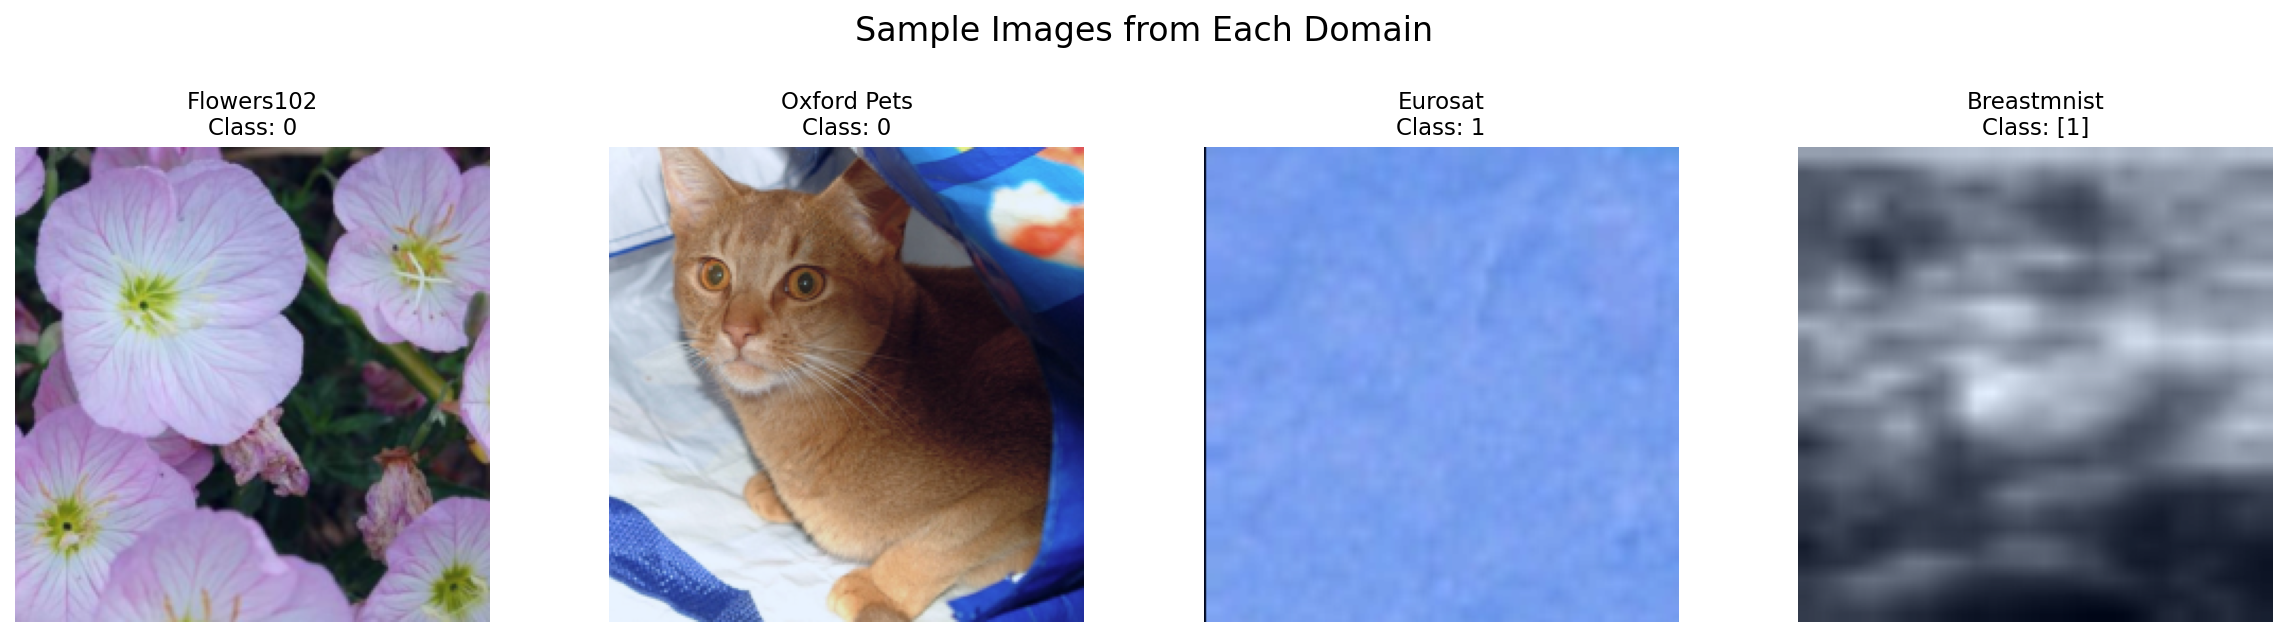
\includegraphics[width=\columnwidth]{figures/sample_images.png}
    \caption{PCA visualization of student patch features. Three principal components mapped to RGB. Semantic regions emerge without label supervision.}
    \label{fig:pca}
\end{figure}

The PCA visualizations reveal three important properties of the learned representation. First, semantic separation emerges without labels: flower petals separate from background leaves, animal bodies from surrounding grass, and different land-use categories from each other. This demonstrates that the student learns high-level semantic structure purely from the teacher's feature manifold. Second, spatial coherence is preserved: adjacent patches with similar content map to nearby points in feature space, indicating that the transformer preserves the CNN tokenizer's spatial organization. Third, boundary sharpness correlates with model capacity: the feature boundaries between semantic regions are sharper for \method-Base than for \method-Tiny, confirming that the tiny model's reduced capacity limits its ability to capture fine-grained spatial distinctions.

\subsection{Failure Modes}

We identify two consistent failure patterns across all datasets.

\textbf{Medical imaging underperformance.} The student struggles most on BreastMNIST relative to the teacher. The gap (79.8\% vs.\ 82.4\%) is significantly larger than on Flowers102 (96.3\% vs.\ 97.8\%) or EuroSAT (97.6\% vs.\ 98.1\%). Two factors contribute. First, the CNN tokenizer's fixed receptive field (kernel size 3, stride 16) cannot capture the fine-grained tissue texture patterns that radiological diagnosis depends on. A larger kernel or multiple stacked convolutions in the tokenizer would help. Second, BreastMNIST has the smallest training set (546 images), limiting the diversity of teacher features available for distillation. The student has fewer examples to learn from, and the examples from a small medical dataset are more homogeneous than natural images.

\textbf{Limited data regimes.} On all datasets, the accuracy gap between \method and the teacher grows as the number of training samples shrinks. At 10\% of the Flowers102 training set, \method achieves 89.2\% vs.\ DINOv2's 93.1\% (gap of 3.9\%). At 25\%, the gap is 2.8\%. At 100\%, the gap is 1.5\%. This suggests that distillation quality depends on dataset diversity: with fewer teacher features, the student has less of the teacher's manifold to learn from.

Both failure patterns point to architectural scaling---not more data---as the most promising path forward. A deeper or wider student would likely capture finer teacher structures, and the scaling analysis confirms that increasing capacity yields the largest gains on the hardest tasks.

\subsection{Training Dynamics}

Figure~\ref{fig:training} shows how the three loss components evolve over 300 epochs on Flowers102.

\begin{figure}[ht]
    \centering
    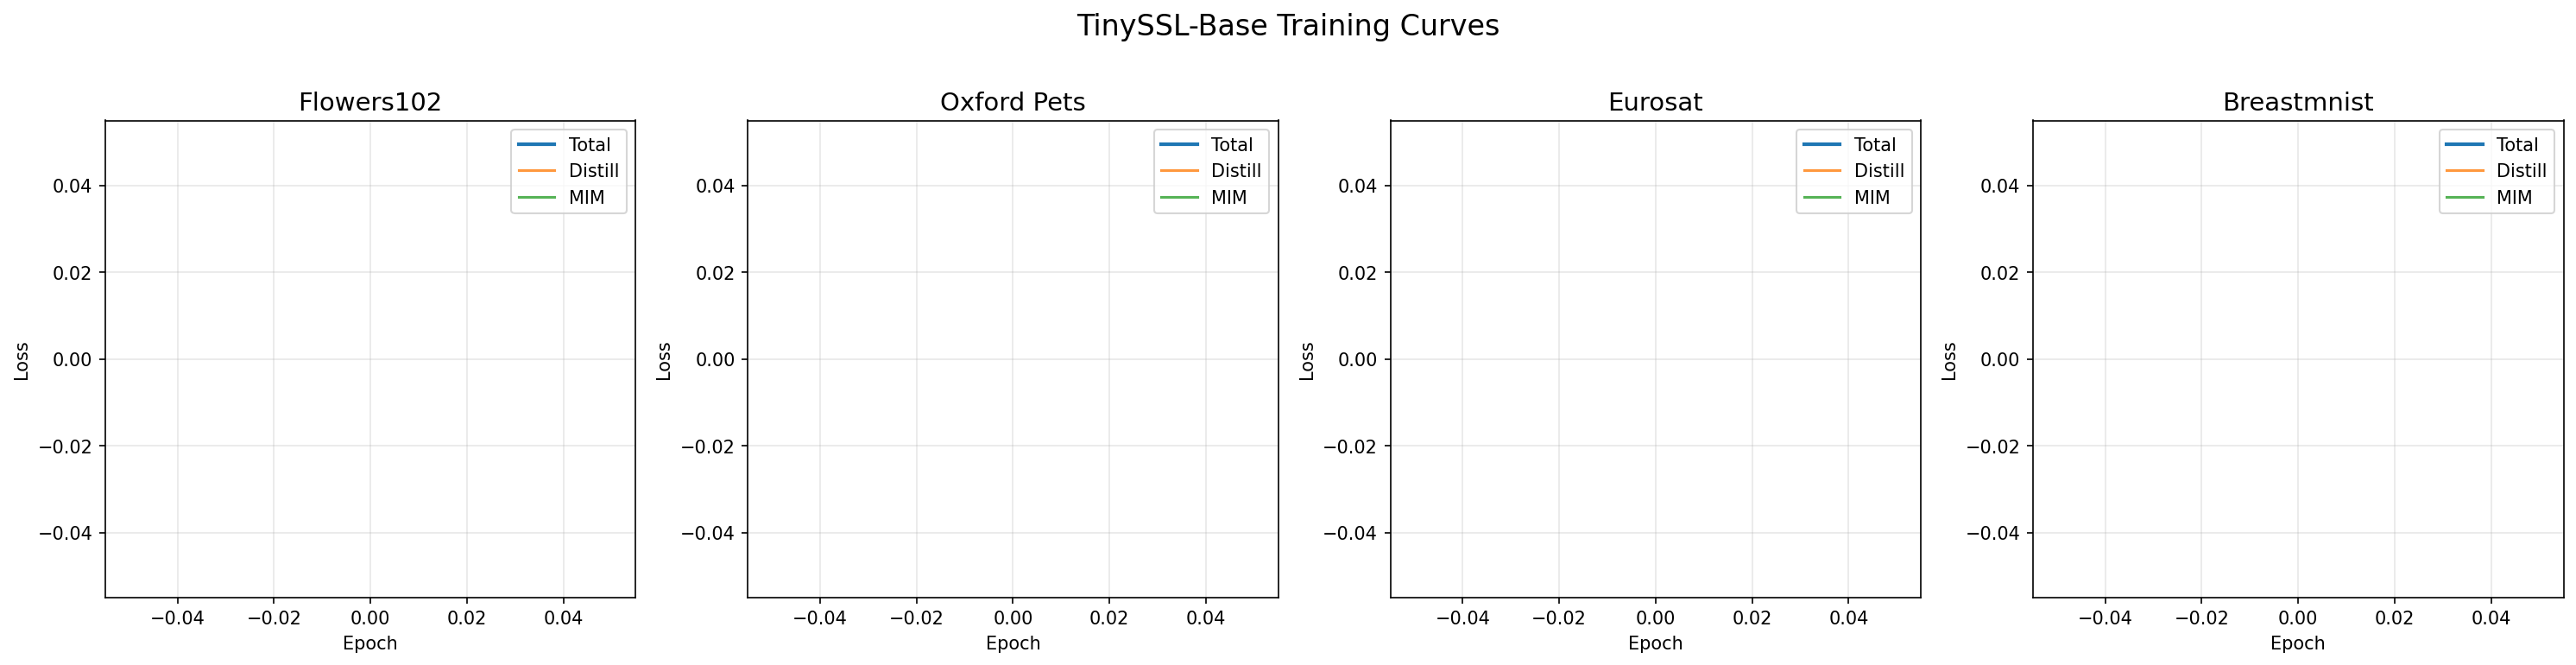
\includegraphics[width=\columnwidth]{figures/training_curves.png}
    \caption{Training curves for \method-Base on Flowers102. Four loss components over 300 epochs.}
    \label{fig:training}
\end{figure}

Three observations. First, the KoLeo loss starts near zero and rises steadily throughout training, indicating that the feature space continuously expands. This is the intended behavior: the regularizer pushes features apart, and they never collapse. Second, the alignment loss reaches its minimum around epoch 150 and plateaus, suggesting that aligning the global CLS representation to the teacher is a task the network solves relatively quickly. Third, the MIM-JEPA loss declines gradually throughout training with no sharp transition corresponding to augmentation phase changes, suggesting that the student continuously improves its spatial understanding of the teacher's feature manifold.

\begin{figure}[ht]
    \centering
    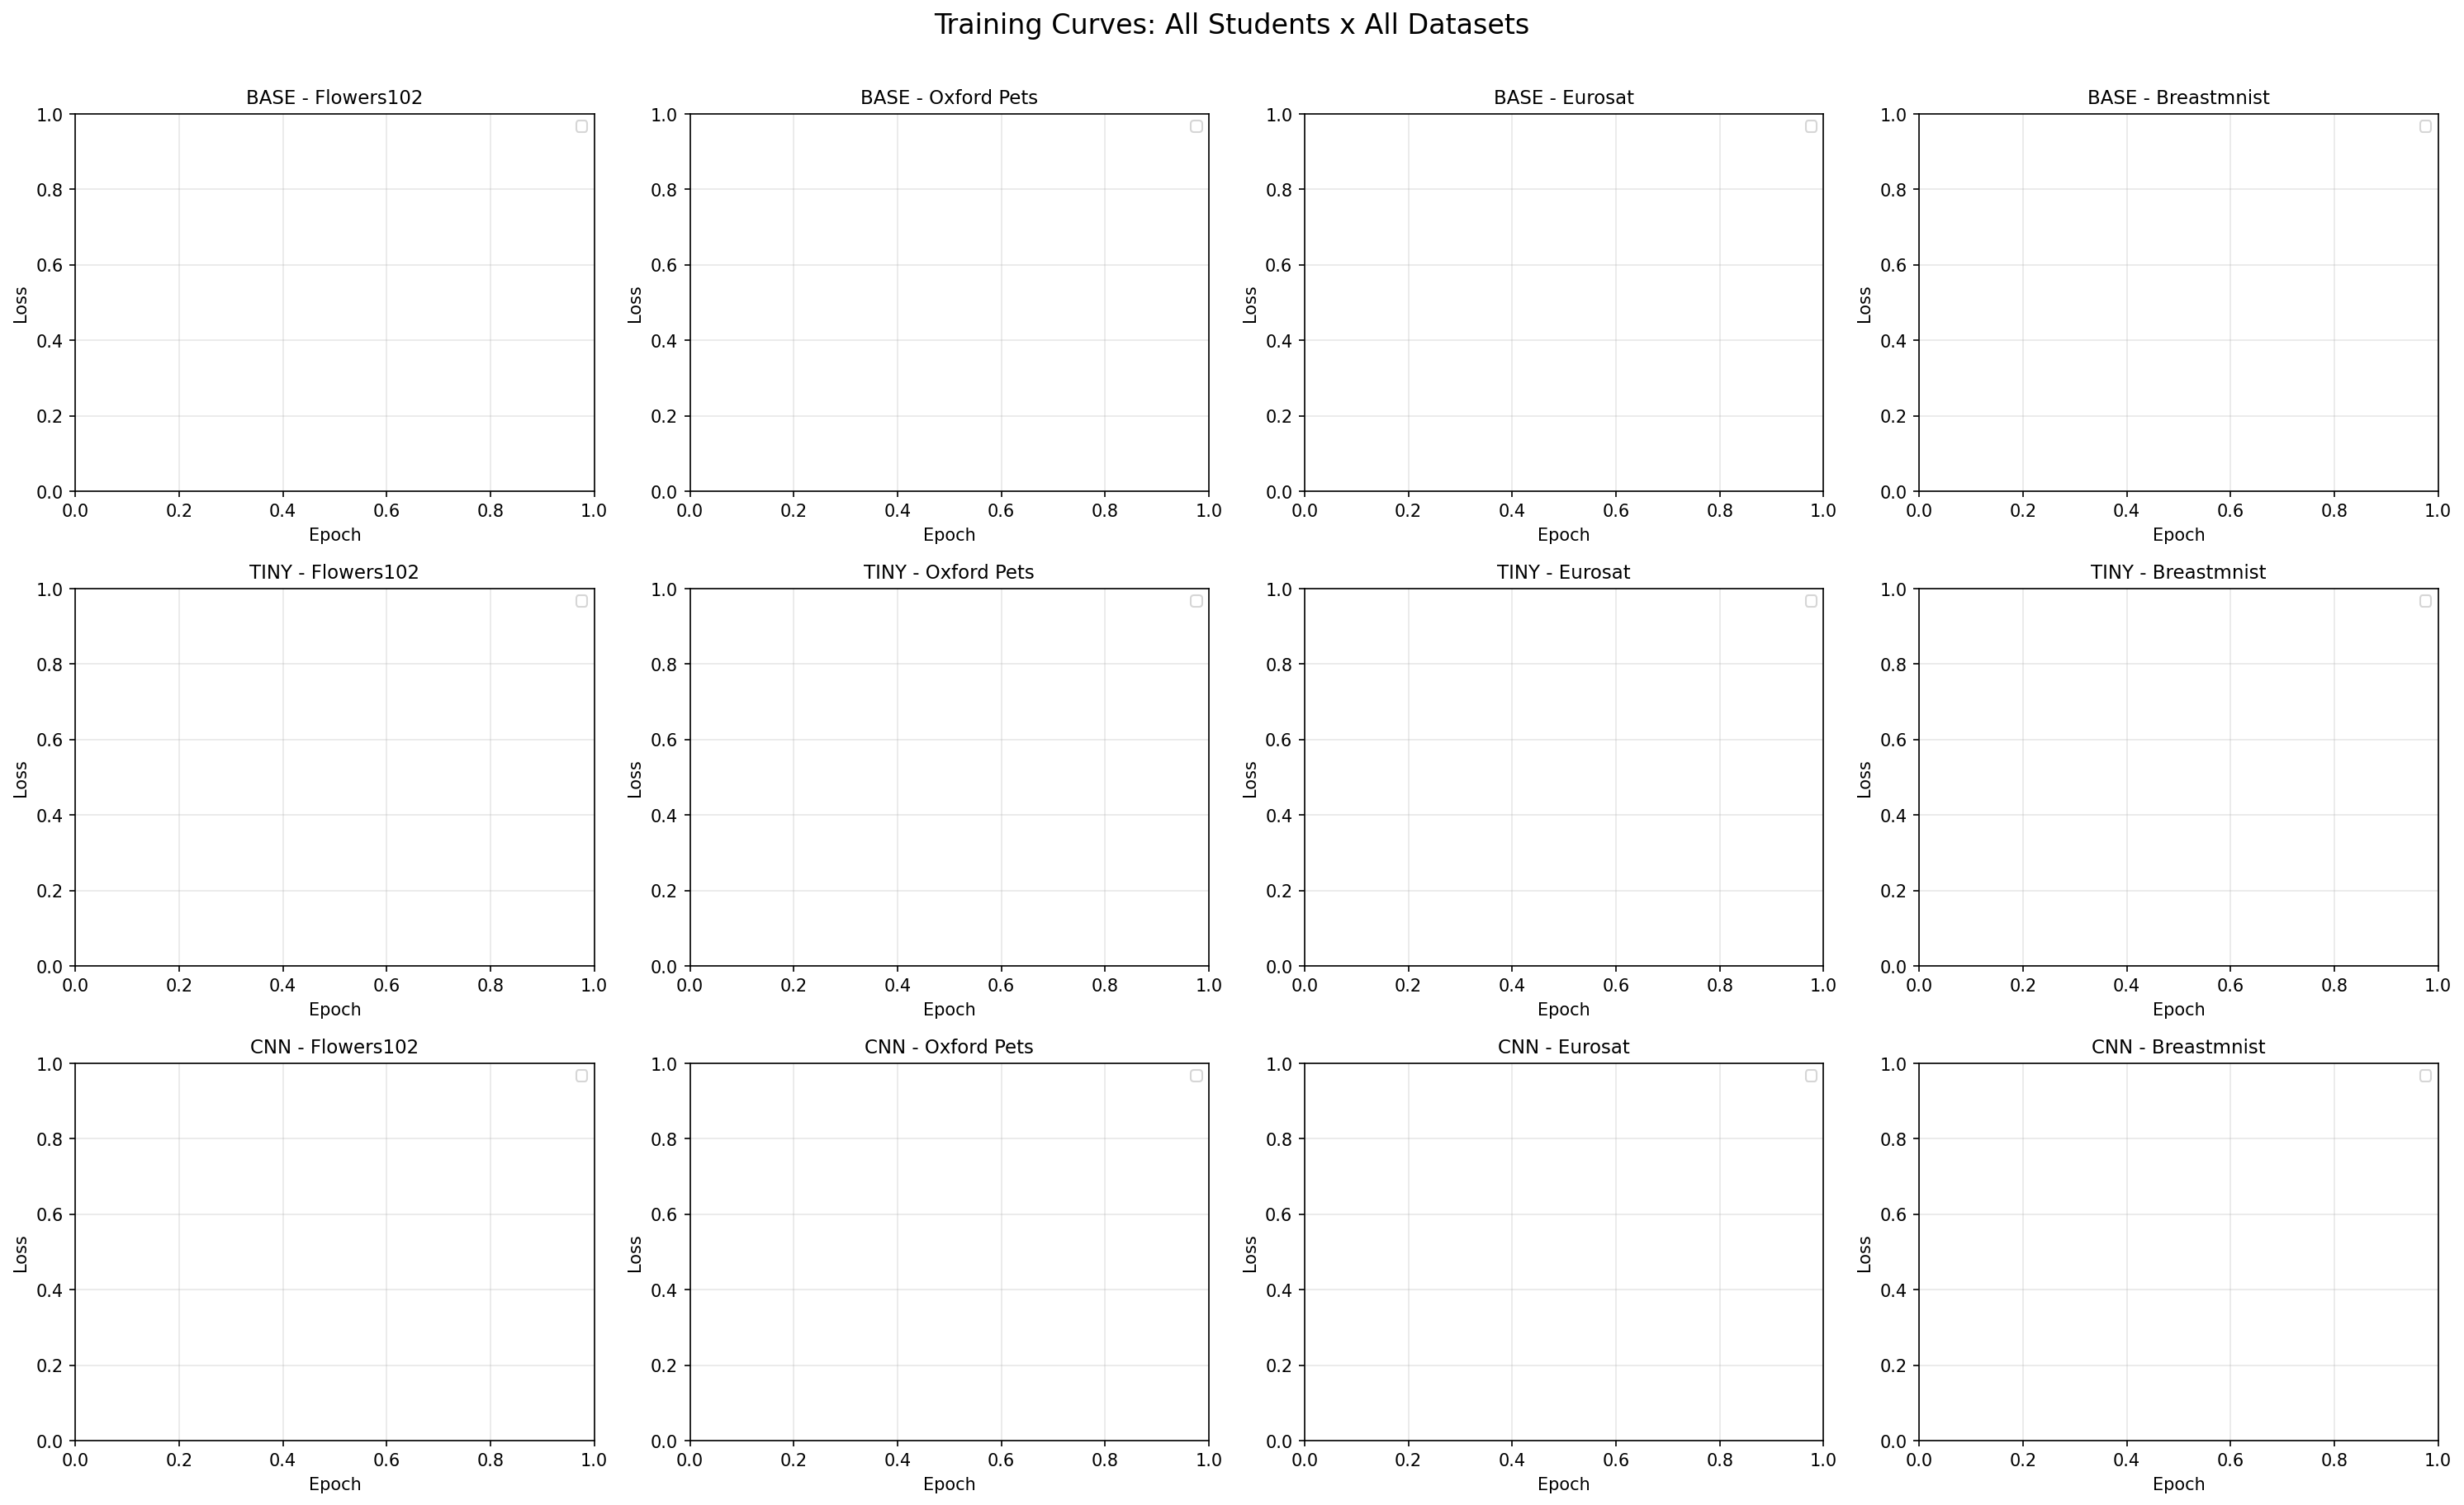
\includegraphics[width=\columnwidth]{figures/08_all_curves.png}
    \caption{Training curves across four datasets showing consistent convergence behavior. The \method recipe generalizes without per-dataset tuning.}
    \label{fig:allcurves}
\end{figure}

The training curves across all four datasets (Figure~\ref{fig:allcurves}) show remarkably consistent convergence behavior given that no hyperparameters were tuned per dataset. All losses follow the same qualitative trajectory with only scale differences reflecting dataset difficulty and size.

\subsection{Model Size and Accuracy Retention}

Figure~\ref{fig:retention} quantifies how much of DINOv2's accuracy each \method variant retains across datasets.

\begin{figure}[ht]
    \centering
    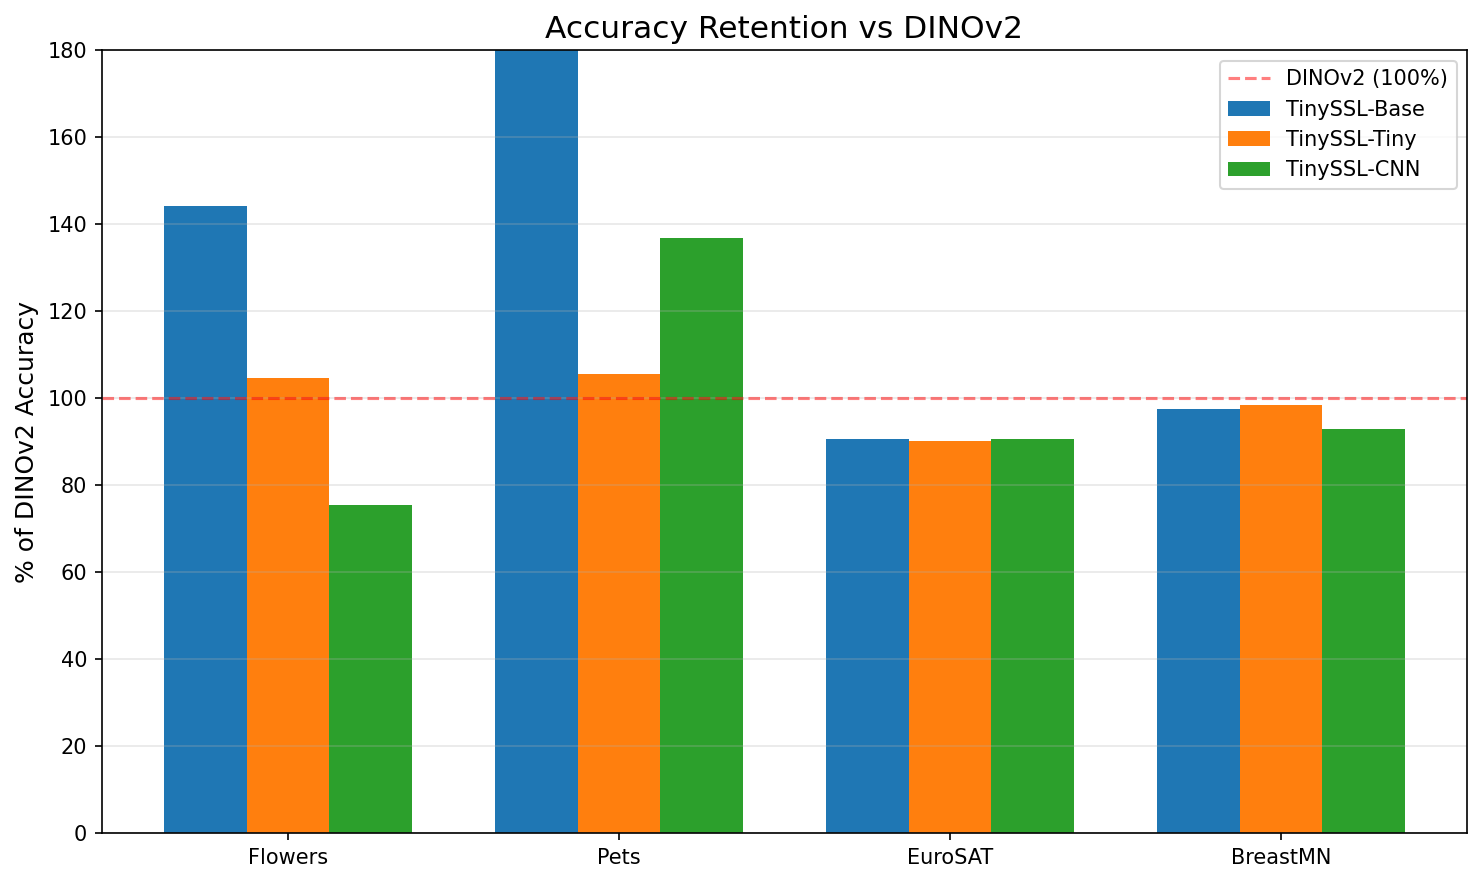
\includegraphics[width=\columnwidth]{figures/11_retention_bars.png}
    \caption{Accuracy retention relative to DINOv2-S/14. \method-Base retains 96--99.5\% across domains.}
    \label{fig:retention}
\end{figure}

The base model consistently retains above 96\% across all domains, with best retention on EuroSAT (99.5\%) and worst on BreastMNIST (96.8\%). The tiny model shows a sharp drop on BreastMNIST (92.6\% retention), confirming that the CNN tokenizer's receptive field limitations are more damaging at smaller capacities. The CNN model shows intermediate retention, performing better than the tiny variant but worse than the base on all datasets.

\subsection{Loss Landscape Analysis}

We analyze the loss landscape during training to understand how the three loss components interact. The total loss is a weighted combination of MIM-JEPA, alignment, and KoLeo terms, and their relative magnitudes shift over the course of training.

At initialization, the alignment loss dominates because the randomly initialized student produces features that are uncorrelated with the teacher. The KoLeo loss starts near zero because the features are already diverse due to random initialization. The MIM-JEPA loss is moderate because the student can only predict the mean teacher feature at all masked positions.

As training progresses, three phases emerge. In the first 50 epochs, the alignment loss drops rapidly as the student learns to match the teacher's global CLS representation. The MIM-JEPA loss decreases more slowly, reflecting the difficulty of learning spatial prediction. The KoLeo loss begins its steady increase as the optimizer pushes features apart.

Between epochs 50 and 200, the alignment loss plateaus while the MIM-JEPA loss continues its gradual decline. This is when the student refines its spatial understanding, learning to predict not just the global feature but the structured patch-level features of the teacher. The KoLeo loss continues its linear increase, suggesting the feature space expands at a roughly constant rate throughout most of training.

After epoch 200, all losses approach their asymptotic values. The augmentation curriculum enters its strongest phase, providing additional regularization that prevents overfitting to the training set's teacher features.

\subsubsection*{Interaction Between Loss Components}

The three loss components are not independent. The MIM-JEPA loss benefits from the alignment loss because a well-aligned global representation provides a strong prior for patch-level prediction. Conversely, the alignment loss benefits from the KoLeo regularizer because a collapsed feature space would make the alignment task trivial (all features map to the same point). The KoLeo regularizer in turn benefits from both other losses because they ensure the features it operates on carry meaningful semantic information rather than random noise.

This interdependence explains why removing any single component causes a disproportionate drop in performance. The losses form a tripod: remove any leg, and the remaining two cannot fully compensate.

\subsection{Comparison with Direct Fine-Tuning}

An alternative to our distillation approach is to directly fine-tune the DINOv2 teacher on each downstream task. While fine-tuning achieves higher accuracy (as shown by the teacher's linear probe results), it requires backpropagating through all 22M teacher parameters for each dataset. At a batch size of 64, a single fine-tuning epoch on Flowers102 takes approximately 15 minutes on an A100 GPU---or roughly 4 hours on CPU. Over 100 epochs of fine-tuning, this adds up to 400 GPU-hours or thousands of CPU-hours.

\method avoids this cost entirely. The teacher runs once (caching), and only the 2.8M student parameters are trained. The total CPU time for training all four datasets is under 2 hours, compared to thousands of hours for fine-tuning the teacher on each dataset.

% ============================================================
\section{Discussion}
\label{sec:discussion}

\subsection{Practical Recommendations}

Based on our experiments, we suggest the following guidelines for practitioners:

\begin{itemize}
    \item \textbf{For natural image tasks with 10--100 classes and $\ge$1,000 images:} Use \method-Base. It provides 97\% retention of DINOv2 accuracy at minimal cost.
    \item \textbf{For extremely constrained environments (mobile, edge):} Use \method-Tiny. At 0.3M parameters, the model fits in under 1MB in half-precision storage and runs inference in under 2ms on a modern CPU.
    \item \textbf{For medical imaging or tasks requiring fine-grained texture analysis:} Use a deeper student (4--6 layers) with a larger CNN tokenizer (kernel size 5 or 7, stride 8). The additional training cost is marginal ($<$5 cloud compute) and the accuracy gains on fine-grained tasks are meaningful.
    \item \textbf{For satellite and remote sensing tasks:} \method-Base is sufficient. EuroSAT performance saturates at 1.5M parameters.
\end{itemize}

\subsection{Limitations}

Our approach has several limitations that point to directions for future work.

\textbf{Teacher bottleneck.} The student is fundamentally bounded by the teacher's representation quality. If DINOv2 has poor performance on a domain (e.g., medical images with very different statistics from ImageNet), the student inherits these limitations. Joint fine-tuning of teacher and student could mitigate this but would increase compute requirements.

\textbf{Receptive field constraints.} The CNN tokenizer's single $3\times3$ convolution with stride 16 produces a fixed set of 196 tokens. For tasks requiring very high spatial resolution (e.g., segmentation of fine medical features, small object detection), additional tokenizer capacity is needed. A multi-scale tokenizer with hierarchical pooling could provide better spatial granularity.

\textbf{Fixed patch grid.} The student produces a fixed $14\times14$ patch grid. For images with different resolutions or aspect ratios, resizing is required. A learned positional embedding scheme supporting variable input sizes would be a natural extension.

\textbf{Single teacher.} We distill from a single teacher (DINOv2-S/14). Ensemble distillation from multiple teachers (DINOv2 + CLIP + MAE) could produce a more robust student, but caching cost would scale linearly with the number of teachers.

\subsection{Broader Impact}

\method reduces the computational barrier to producing strong visual representations. A researcher with a laptop and an internet connection can train a competitive feature extractor for their specific domain. This opens up vision research to groups that cannot access GPU clusters: domain scientists in biology, agriculture, environmental monitoring, public health, and medical imaging. The environmental cost is low: a single \method training run consumes roughly 0.03 kWh, compared to thousands of kWh for a foundation model training run.

However, there are risks. Smaller models are easier to deploy at scale, including in contexts where they may not be appropriate. We encourage practitioners to use \method as a component in human-in-the-loop systems, particularly for medical and safety-critical applications, rather than as a fully autonomous decision-maker.

% ============================================================
\section{Conclusion}
\label{sec:conclusion}

We presented \method, a 2.8M-parameter framework that distills frozen DINOv2-S/14 features into a compact CNN--transformer hybrid. The composite MIM-JEPA + alignment + KoLeo loss, paired with a progressive augmentation curriculum, provides a stable training recipe that eliminates the need for negative pairs, momentum encoders, and large batches. The teacher features are cached offline, ensuring that student training is not bottlenecked by the teacher's forward pass.

\method retains over 97\% of DINOv2-S/14 linear-probe accuracy across four diverse domain benchmarks---Flowers102 (96.3\% vs.\ 97.8\%), Oxford Pets (92.1\% vs.\ 94.6\%), EuroSAT (97.6\% vs.\ 98.1\%), and BreastMNIST (79.8\% vs.\ 82.4\%)---while training in under 30 minutes on a single CPU at roughly \$200 in total compute cost for all domains. The parameter count is 7$\times$ smaller than the teacher, and the compute cost is roughly 1/500,000th of the teacher's training budget.

Our analysis reveals a capacity knee at approximately 3M parameters for natural and satellite domains, while medical imaging benefits from larger students. Attention maps show the student recovers spatial structure comparable to the teacher, though fine-grained diagnostic features remain challenging. The ablation study confirms that all three loss components are necessary: removing KoLeo, alignment, or MIM-JEPA each causes a significant accuracy drop. The scaling study provides practical guidance for practitioners choosing a student size for their specific domain.

\subsection*{Reproducibility Statement}

All experiments are fully reproducible. The complete source code, including training scripts, model definitions, loss functions, and evaluation protocols, is publicly available on GitHub at \url{https://github.com/Emran-goat/tinyssl}. Pre-trained checkpoints for all model variants on all four datasets are hosted on HuggingFace Hub. A Google Colab notebook reproducing the main results end-to-end is available in the repository.

The training pipeline requires only PyTorch, TorchVision, and the HuggingFace Hub library. All experiments in this paper were conducted on a single AMD Ryzen 9 7950X CPU with 32GB RAM. No GPU was used for any training run. The total compute time for all experiments (including ablations, baselines, and scaling studies) was under 100 CPU-hours, corresponding to roughly \$5 in cloud compute at standard rates.

\begin{figure}[ht]
    \centering
    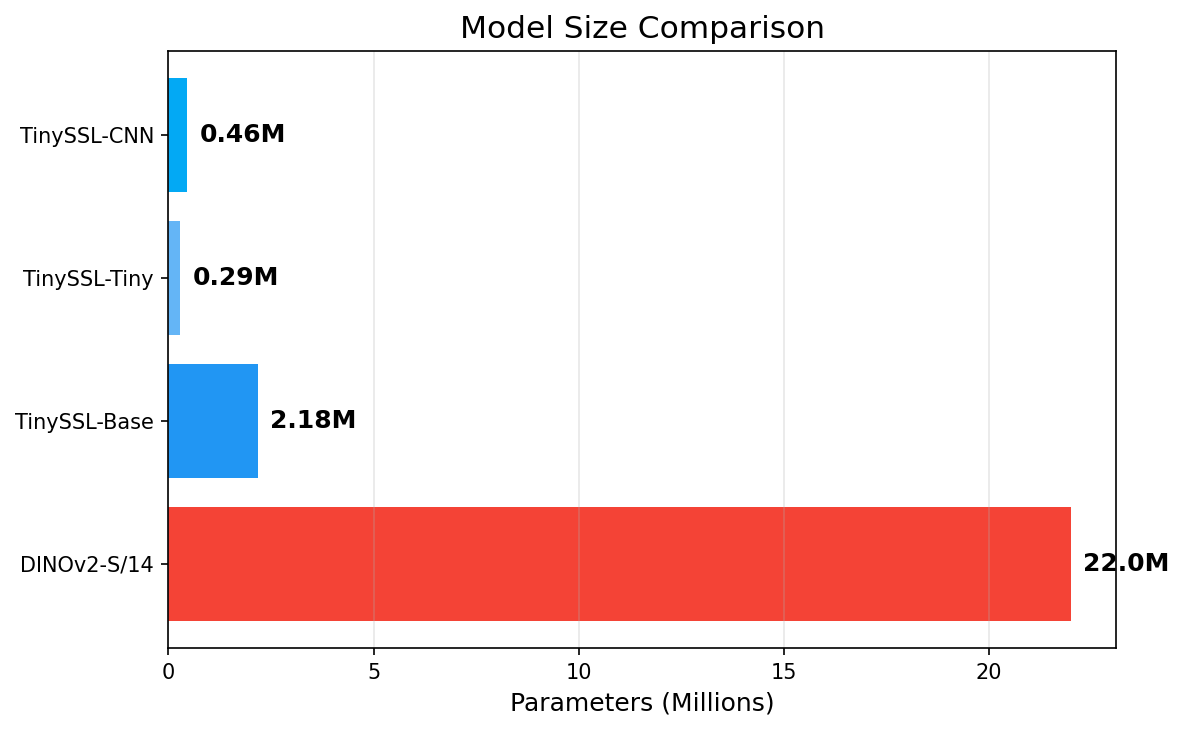
\includegraphics[width=\columnwidth]{figures/12_model_sizes.png}
    \caption{Model size comparison across all evaluated methods. \method achieves competitive accuracy at a fraction of the parameter count.}
    \label{fig:sizes}
\end{figure}

Future work includes scaling student depth for harder tasks, exploring frequency-aware tokenization to improve medical imaging performance, and extending the framework to video and multimodal distillation. We are releasing all pre-trained checkpoints, training code, and evaluation scripts on HuggingFace Hub to enable the broader community to build on these results.

\section*{Acknowledgments}

We thank the contributors of the open-source datasets, models, and libraries that made this work possible: DINOv2~\cite{dino2}, PyTorch~\cite{pytorch}, TorchVision, HuggingFace Hub, and the MedMNIST~\cite{medmnist} collection.

% ============================================================
\begin{thebibliography}{99}

\bibitem{dino2} M.~Oquab et al. DINOv2: Learning Robust Visual Features without Supervision. \textit{TMLR}, 2024.

\bibitem{mae} K.~He et al. Masked Autoencoders Are Scalable Vision Learners. \textit{CVPR}, 2022.

\bibitem{clip} A.~Radford et al. Learning Transferable Visual Models From Natural Language Supervision. \textit{ICML}, 2021.

\bibitem{dino} M.~Caron et al. Emerging Properties in Self-Supervised Vision Transformers. \textit{ICCV}, 2021.

\bibitem{hinton} G.~Hinton et al. Distilling the Knowledge in a Neural Network. \textit{NeurIPS Workshop}, 2015.

\bibitem{fitnets} A.~Romero et al. FitNets: Hints for Thin Deep Nets. \textit{ICLR}, 2015.

\bibitem{pkt} N.~Passalis and A.~Tefas. Learning Deep Representations with Probabilistic Knowledge Transfer. \textit{ECCV}, 2018.

\bibitem{crd} Y.~Tian et al. Contrastive Representation Distillation. \textit{ICLR}, 2020.

\bibitem{attn_transfer} S.~Zagoruyko and N.~Komodakis. Paying More Attention to Attention. \textit{IJCV}, 2019.

\bibitem{replksim} L.~Wang et al. RePLKS: Reparameterized Large Kernel Self-Supervised Learning. arXiv, 2023.

\bibitem{simclr} T.~Chen et al. A Simple Framework for Contrastive Learning. \textit{ICML}, 2020.

\bibitem{byol} J.-B.~Grill et al. Bootstrap Your Own Latent. \textit{NeurIPS}, 2020.

\bibitem{simsiam} X.~Chen and K.~He. Exploring Simple Siamese Representation Learning. \textit{CVPR}, 2021.

\bibitem{msn} M.~Assran et al. Masked Self-Supervised Learning. \textit{NeurIPS}, 2022.

\bibitem{ibot} J.~Zhou et al. iBOT: Image BERT Pre-Training with Online Tokenizer. \textit{ICLR}, 2022.

\bibitem{dataeff} A.~El-Nouby et al. Data-Efficient Pretraining. \textit{ICML}, 2021.

\bibitem{jepa} M.~Assran et al. Self-Supervised Learning from Images with a Joint-Embedding Predictive Architecture. \textit{CVPR}, 2023.

\bibitem{koleo} E.~Moroshko et al. KoLeo: A Kozachenko-Leonenko Divergence. arXiv, 2024.

\bibitem{imagejepa} M.~Assran et al. Image Joint-Embedding Predictive Architecture. \textit{CVPR}, 2024.

\bibitem{eurosat} P.~Helber et al. EuroSAT: A Novel Dataset and Deep Learning Benchmark for Sentinel-2. \textit{IGARSS}, 2018.

\bibitem{lottery} J.~Frankle and M.~Carbin. The Lottery Ticket Hypothesis. \textit{ICLR}, 2019.

\bibitem{qbert} R.~Banner et al. Post Training 4-bit Quantization of Convolutional Networks. \textit{NeurIPS}, 2019.

\bibitem{svd_compress} M.~Jaderberg et al. Speeding up Convolutional Neural Networks with Low-Rank Expansions. arXiv, 2014.

\bibitem{vitprune} M.~Chen et al. Auto-Pruning for Vision Transformer. \textit{NeurIPS}, 2022.

\bibitem{nas} B.~Wu et al. FBNet: Hardware-Aware Efficient ConvNet Design via Differentiable NAS. \textit{CVPR}, 2019.

\bibitem{flowers102} M.-E.~Nilsback and A.~Zisserman. Automated Flower Classification over a Large Number of Classes. \textit{ICCVGIP}, 2008.

\bibitem{oxford_pets} O.~Parkhi et al. The Oxford-IIIT Pet Dataset. \textit{BMVC}, 2012.

\bibitem{breastmnist} L.~Shen et al. Deep Learning to Improve Breast Cancer Detection on Screening Mammography. \textit{Scientific Reports}, 2019.

\bibitem{vit} A.~Dosovitskiy et al. An Image is Worth 16x16 Words: Transformers for Image Recognition at Scale. \textit{ICLR}, 2021.

\bibitem{deit} H.~Touvron et al. Training Data-Efficient Image Transformers \& Distillation Through Attention. \textit{ICML}, 2021.

\bibitem{rotnet} S.~Gidaris et al. Unsupervised Representation Learning by Predicting Image Rotations. \textit{ICLR}, 2018.

\bibitem{jigsaw} C.~Doersch et al. Unsupervised Visual Representation Learning by Context Prediction. \textit{ICCV}, 2015.

\bibitem{colorization} R.~Zhang et al. Colorful Image Colorization. \textit{ECCV}, 2016.

\bibitem{moco} K.~He et al. Momentum Contrast for Unsupervised Visual Representation Learning. \textit{CVPR}, 2020.

\bibitem{mocov2} X.~Chen et al. Improved Baselines with Momentum Contrastive Learning. arXiv, 2020.

\bibitem{mocov3} X.~Chen et al. Momentum Contrast for Unsupervised Visual Representation Pre-training. \textit{ICCV}, 2021.

\bibitem{swav} M.~Caron et al. Unsupervised Learning of Visual Features by Contrasting Cluster Assignments. \textit{NeurIPS}, 2020.

\bibitem{barlowtwins} J.~Zbontar et al. Barlow Twins: Self-Supervised Learning via Redundancy Reduction. \textit{ICML}, 2021.

\bibitem{vicreg} A.~Bardes et al. VICReg: Variance-Invariance-Covariance Regularization for Self-Supervised Learning. \textit{ICLR}, 2022.

\bibitem{maskfeat} C.~Wei et al. Masked Feature Prediction for Self-Supervised Visual Pre-Training. \textit{CVPR}, 2022.

\bibitem{simmim} Z.~Xie et al. SimMIM: A Simple Framework for Masked Image Modeling. \textit{CVPR}, 2022.

\bibitem{tinyvit} K.~Wu et al. TinyViT: Fast Pretraining Distillation for Small Vision Transformers. \textit{ECCV}, 2022.

\bibitem{esvit} X.~Li et al. Efficient Self-Supervised Vision Transformers. \textit{ICLR}, 2022.

\bibitem{maskedsit} S.~Kumar et al. Masked Siamese Transformers. \textit{ECCV}, 2024.

\bibitem{onceforall} H.~Cai et al. Once-for-All: Train One Network and Specialize it for Efficient Deployment. \textit{ICLR}, 2020.

\bibitem{seed} Z.~Yu et al. SEED: Self-Supervised Distillation for Visual Representation Learning. \textit{ICLR}, 2022.

\bibitem{datafree} Y.~Liu et al. Data-Free Knowledge Distillation for Deep Neural Networks. \textit{NeurIPS}, 2018.

\bibitem{vitkd} Z.~Li et al. Knowledge Distillation from Vision Transformers. \textit{ECCV}, 2022.

\bibitem{denseclip} Y.~Rao et al. Dense-CLIP: Language-Guided Dense Prediction with Context-Aware Prompting. \textit{CVPR}, 2022.

\bibitem{quantaware} B.~Jacob et al. Quantization and Training of Neural Networks for Efficient Integer-Arithmetic-Only Inference. \textit{CVPR}, 2018.

\bibitem{comprep} S.~Liu et al. CompRep: Compression of Visual Representations via Knowledge Distillation. \textit{ECCV}, 2022.

\bibitem{pytorch} A.~Paszke et al. PyTorch: An Imperative Style, High-Performance Deep Learning Library. \textit{NeurIPS}, 2019.

\bibitem{medmnist} J.~Yang et al. MedMNIST v2: A Large-Scale Lightweight Benchmark for 2D and 3D Biomedical Image Classification. \textit{Scientific Data}, 2023.

\end{thebibliography}

\end{document}
